\documentclass[a5paper,14pt]{book}
\usepackage{abyz}
\usepackage[colorlinks,linkcolor=black,citecolor=black]{hyperref}
\usepackage{graphicx}
\usepackage{amsthm,amssymb}
\usepackage{tocbibind}
\usepackage{listings}
\usepackage{xepersian}
\usepackage{longtable}
\settextfont[Scale=1]{B Nazanin}
\setlatintextfont[Scale=1]{Liberation Serif}

\author{نویسنده:آلبرتو ساویا
\\ مترجم: عباس یزدان‌پناه}
\title{پیش‌نمونه سازی
\\
مطمئن شوید که شما در حال ساختن  آن چیز درست هستید قبل از اینکه شروع به ساختن آن چیز نمایید}
\makeindex
\begin{document}
\maketitle
\frontmatter
\tableofcontents

\chapter{این خجالت آور است}
این یک کتاب به شکل معمول نیست.

نوشتن و ویرایش یک کتاب به شکل معمول در مورد پیش‌نمونه سازی ماه‌ها زمان
خواهد برد. من دوست دارم اینچنین کتابی به نویسم اما در حال حاضر نشانه‌ای
بر ارزشمند بودن نوشتن چنین کتابی وجود ندارد. بیشتر کتاب‌ها در بازار شکست
می‌خورند، و دلیل شکست اکثر آنها این نیست که به درستی نوشته نشده یا
ویرایش شده نشده‌اند، بلکه به این دلیل است که افراد کمی به آنها علاقه‌مند
هستند. آنها \emph{یک} \textbf{چیز} \emph{درست} نیستند.

کتابی که پیش روی شماست نسخه پیش‌نمونه‌ی کتاب است. من این کتاب را در عرض
چند روز نوشتم و «ویرایش» کردم بجای چند ماه، به منظور اینکه سطح علاقه به
این کتاب را دریابم. برخی از دوستان و همکاران من این کتاب را بررسی
کرده‌اند اما اگر در این کتاب غلط املایی، دستور زبان نادرست و هرگونه
\emph{ایراد} دیگر پیدا کردید تعجب نکنید.

نشر این کتاب در این وضعیت برای من آسان نیست.

سخت ترین بخش در مورد پیش‌نمونه سازی توسعه پیش‌نمونه ها نیست زیرا این بخش
لذتبخش است. سخت ترین بخش غلبه بر میل شدید به ایده‌آل گرایی و همچنین
علاقه به اضافه کردن ویژگی و یا محتوا قبل از انتشار اولیه است. بخش سخت
عرضه پیش‌نمونه در مقابل دیگران است و این در حالی است که ممکن است مورد آن
قضاوت شود، مورد نقد قرار بگیرد و یا بصورت محتمل ترد گردد.

رید هافمن -یکی از پایه گذاران لینکدین- می‌گوید: «اگر شما از اولین نسخه
محصول خود خجالت نمی‌کشید شما خیلی دیر نسخه اولیه را ارائه کرده‌اید»

من خیلی خجالت میکشم، پس من باید مسیر درستی را انتخاب کرده باشم.

\chapter{مقدمه}
هم‌اینک، میلیون‌ها انسان در سراسر دنیا قلب، روح، امیدها، آرزوها، زمان،
پول و انرژی خود را صرف توسعه ایده‌های جدیدی می‌کنند که به محض راه‌اندازی
به شکل ناراحت‌کننده‌ای شکست می‌خورند.

همچنین در همین لحظه، تعداد بسیار کمتری در حال توسعه ایده‌های جدید هستند
که موفق خواهند شد. برخی از آنها حتی بسیار موفق شده و آیپاد بعدی، گوگل
بعدی، توییتر بعدی خواهند بود.

شما در کدام گروه هستید؟

بسیاری بر این باورند که در حال کار روی محصول برنده هستند، اما میدانیم که
این نمیتواند درست باشد.

بیشتر ایده‌های جدید شکست می‌خورند و پیش‌بینی موفقیت در بازار ایده‌ی جدید
با درجه‌ای از اطمینان تقریبا غیرممکن است. بسیاری از ایده‌های «\emph{شکست
ناپذیر}» شکست‌های بزرگی از آب در می‌آیند. در حالی که برخی ایده‌های جنون
آمیز «\emph{کی اینو میخواد؟}» موفقیت‌های تماشایی می‌شوند.

بعضی از افراد و برخی از شرکت‌ها ممکن است از دیگران توان بهتری در
پیش‌بینی موفقیت داشته باشند، اما بهترین سرمایه‌گذاران ریسک پذیر، سرمایه
گذاران و کارآفرینان بطور مرتب سرمایه بیش از حدی روی \emph{ایده‌های غلط}
گذاشته و مرتبا بصورت فعالی روی \emph{ایده درست} سرمایه گذاری نمی‌کنند.

اگه همه ما \emph{ایده‌ای} برای یک محصول جدید(یا سرویس، یا کتاب و موارد
مشابه) داریم، بهرتین کاری که می‌توانیم انجام دهیم جمع آوری \emph{نظرات}
در مورد کاربردی بودن و پتانسیل بازار است. ایده‌ها فازی و انتزاعی هستند.
نظرات ذهنی بوده و حتی بیشتر از ایده‌ها انتزاعی هستند. وقتی شما این دو را
با هم ترکیب می‌کنید یک مجموعه بزرگ فازی از انتزاعات و نظرات دارید. چیزی
زیادی برای ادامه دادن وجود ندارد.

نمونه‌های اولیه می‌توانند بجای ایده‌ها و نظرات به تست و ارزیابی پتانسیل
بازار یک ایده جدید بصورت درست و عینی کمک کنند. اما در بسیاری از موارد،
توسعه یک «نمونه اولیه مناسب» بسیار سخت، پرهزینه و زمانبر است. این مساله
عادی است هفته‌ها، ماه‌ها یا سال‌ها زمان و صدها، هزاران و حتی میلیون‌ها
دلار برای توسعه یک نمونه اولیه صرف شود. همچنین، نمونه‌های اولیه برای
پاسخ به سوالاتی همانند «آیا می‌توانیم این را بسازیم؟» یا «این به
همانگونه که مورد انتظار است عمل می‌کند» ساخته می‌شوند و تاکیدی بر «آیا
بایستی این را اصلا بسازیم؟» یا «اگر این را بسازیم، آیا مردم آنرا می‌خرند
و از آن استفاده میکنند؟» ندارند. اگر شما بتوانید با نمونه اولیه به دو
سوال آخر جواب مثبت بدهید، دو سوال اول از درجه اهمیت کمی برخوردارند.

نمونه‌های اولی به شما کمک می‌کنند که زودتر شکست بخورید، اما این شکست به
اندازه کافی سریع و کم هزینه نیست. هرچه بیشتر روی چیزی سرمایه گذاری کنید
سختر می‌توانید از آن دست کشیده و قبول کنید که این چیز غلط است. وقتی شما
یک «نمونه اولیه مناسب» داشته باشید، کمی بیشتر روی آن کار کردن و بیشتر
روی آن سرمایه گذاری کردن اغوا کننده است: «اگر ما ین ویژگی را اضافه کنیم،
من مطمئنم مردم از آن استفاده خواهند کرد». نمونه‌های اولیه معمولا تبدیل
به \emph{محصولات اولیه} (نمونه‌های اولیه‌ای که روی آنها زمان بیش از حدی
گذاشته شده) و شما می‌تواند یک شکست سریع را تجربه کنید.

مرحل میانی بین ایده‌های انتزاعی و «نمونه‌‌ی اولیه مناسب» \emph{پیش
نمونه} است. این پیش نمونه‌ها امکان جمع آوری اطلاعات ارزشمند مربوط به
نحوه استفاده و بازار را برای شروع و یا عدم شروع یک ایده جدید را فراهم
می‌کنند. این اطلاعات در پیش‌نمونه‌ها در کسری از هزینه نسبت به نمونه‌های
اولیه بدست می‌آید : ساعت‌ها یا روزها بجای هفته‌ها یا ماه‌ها و چند پنی
بجای چند دلار. پیش نمونه‌ها به شما کمک می‌کنند که به سرعت شکست خورده و
سریع بهبود بیابید. و زمان، پول، انرژی و اشتیاق کافی برای کاوش ترفند‌ها و
ایده‌های جدید در اختیار شما قرار می‌دهد. تا زمانی که ایده‌ای بیابید که
به نظر موافق طبع مردم است، همان «\emph{یک} \textbf{آن} \emph{درست}» نادر
و شگفت انگیز.

بسیاری از مواردی که در این کتاب می‌خوانید به نظر شما واضح می‌آید. اما
قبل از عبور سریع از روی آنها، نگاهی به محصولات، سرویس‌ها، نرم‌افزارها،
کتاب‌ها و غیره اطراف خود انداخته که هرروز ارائه شده و خیلی زودهم شکست
می‌خورند. دلیل شکست اکثر این محصولات بخاطر این نیست که افرادی که آنها را
تولید کرده‌اند نادان، تنبل یا بی‌کفایت بودند. همچنین این شکست به دلیل
کیفت پایین ساخت محصولات و بازاریابی آنها نیست. این شکست بخاطر درست نبودن
محصولی است که آنها کار را با آن شروع کرده‌اند.

این شانس وجود دارد که شما به گذشته خود نگاه کرده و محصولات را که روی آن
کار کرده‌اید بیابید تشخیص بدهید که با گذشت زمان معلوم شده است که آنها
محصولات درستی نبوده‌اند مگر اینکه شما به تازگی دوره کاری خود را آغاز
کرده باشید. این دقیقا در مورد من صدق میکند. من شانس کار کردن روی
محصولاتی را داشته ام که ماه‌ها کار را تبدیل به میلیونها(حتی میلیاردها)
کرده و همچنین روی محصولاتی که سالها کار و ده‌ها میلیون را تبدیل به
«خاکستر» کرده است.

با وجود اینکه این نسخه کتاب به خودی خود یک پیش نمونه است(من بعدا در این
مورد بیشتر توضیح خواهم)، بایستی ارزش کافی برای وقت شما را داشته باشد. من
خالصانه از این حقیقت که شما این کتاب را میخوانید قدردانی میکنم. لطفا
نظرات خود را برای من بفرستید - من نیاز به اطلاعات برای فهمیدن درستی
سرمایه‌گذاری برای تبدیل این پیش کتاب به یک کتاب مناسب دارم.

با تشکر از شما

آلبرتو ساویا(asavoia@gmail.com) آگوست 2011

ترجمه: عباس یزدان پناه ژانویه 2015

\mainmatter
\chapter{آن چیز درست}
عنوان این این کتاب «؟؟» بوده و زیر عنوان کتاب «مطمئن شوید که شما در حال
ساختن \emph{آن} \textbf{چیز} \emph{درست} هستید قبل از اینکه شروع به
ساختن آن \textbf{چیز} نمایید.»

من خیلی زود پیش نمونه‌سازی را توصیف و تعریف خواهم کرد. اما قبل از آن، ما
نیاز به بررسی این سوال داریم که:

این \textbf{چیزی} که من از آن صحبت می‌کنم چیست؟ و چرا اینقدر داشتن
«\emph{آن} \textbf{چیز} \emph{درست}» مهم است؟

\section{این \textbf{چیزی} که من از آن صحبت می‌کنم
چیست؟}\label{ux627ux6ccux646-ux686ux6ccux632ux6cc-ux6a9ux647-ux645ux646-ux627ux632-ux622ux646-ux635ux62dux628ux62a-ux645ux6ccux6a9ux646ux645-ux686ux6ccux633ux62a}

در کل این کتاب، آن \textbf{چیز} می‌واند یک محصول،یک سرویس،یک کتاب،یک کسب
و کار نوپا، یک نهاد خیریه، یک بازی کامپیوتری، یک نوع خلاقانه از قایق، یک
ساز موسیقی، یک همستر ضد حساسیت مهندسی ژنیتیک شده و \ldots{} جدید باشد.

این \textbf{چیز} ممکن است حتی تا کنون وجود نداشته باشد، اما شما در حال
فکر کردن درباره آن بوده و علاقه مند یا مجبور به ساختن آن و حیات بخشیدن
به آن باشید.

این \textbf{چیز} ممکن است برای شما مهم باشد، و ساختن این \textbf{چیز}
نیازمند بخش بزرگی از زمان، تلاش و سرمایه شما بوده و همچنین نیازمند بخش
قابل توجهی از انرژی، انگیزه، اشتیاق و تعهد شما باشد.

بصورت ایده‌آل، این \textbf{چیز} یکی از مواردی است که شما عمیقا در مورد
آن علاقه‌مند هستید، اما اگر این \textbf{چیز} تنها بخشی از کار شماست نیز
قابل قبول است.

\section{چرا اینقدر داشتن «\emph{آن} \textbf{چیز} \emph{درست}» مهم
است؟}\label{ux686ux631ux627-ux627ux6ccux646ux642ux62fux631-ux62fux627ux634ux62aux646-ux622ux646-ux686ux6ccux632-ux62fux631ux633ux62a-ux645ux647ux645-ux627ux633ux62a}

ابر و باد و مه و خورشید فلک به شدت بر علیه موفقیت این \textbf{چیز} شما
هستند. امیدوارم این خبر جدید برای شما نباشد. مطمئنم که آمارهای مشابه این
آمارهای شنیده‌اید: - ۹۰ درصد نرم‌افزارهای موبایل اصلا درآمدی ندارند. -
از هر پنج کسب و کار نوپا چهار تای آنها سرمایه‌ی سرمایه‌گذاران خود را از
دست می‌دهند. - ۸۰ درصد رستوران‌های جدید در یک سال اول تعطیل می‌کنند.

بیشتر \textbf{چیز}های جدید شکست می‌خورند. بدشانسی‌های شما همانند دیگران
است مگر اینکه شما قدرت ماورایی تغییر تقدیر را داشته باشید. احتمال شکست
آن \textbf{چیز} شما که الان به آن فکر می‌کنید زیاد است. مگر اینکه آن
\textbf{چیز} شما یکی از \emph{آن} \textbf{چیز} \emph{درست} نایاب باشد.

اگر شما \emph{آن} \textbf{چیز} \emph{درست} را نداشته باشید پس قاعدتا
بایستی \emph{آن} \textbf{چیز} \emph{غلط} را داشته باشید. یکی از
بی‌فایده‌ترین و پرهزینه‌ترین کارهایی که می‌توانید انجام دهید ادامه کار
روی \textbf{چیز} \emph{غلط} و تلاش برای موفق کردن آن به کمک تلاش و نیروی
اراده است. متاسفانه موفقیت \textbf{چیز} غلط با تلاش زیاد بسیار نادر بوده
و گفته می‌شود که آن \textbf{چیز} \emph{غلط} با هر میزان زمان و هزینه
درست نمی‌شود.

فیلم‌ها نمونه خوبی از غیر ممکن بودن تبدیل آن \textbf{چیز} \emph{غلط} به
یک فیلم پرفروش در گیشه‌هاست. اگر ایده فیلم(آن \textbf{چیز} در این حالت)
درست نباشد، استفاده از کارگردانان و بازیگران مشهور و بودجه بالا ۱۰۰
میلیون دلار باعث موفقیت فیلم نمی‌شود(به عنوان مثال فیلمّای «ایشتار»،
«دروازه بهشت»،«هاوارد اردک»).

در عین حال، اگر شما آن \textbf{چیز} \emph{درست} را داشته باشید، همه چیز
راحت‌تر بوده و ابر و باد و مه و خورشید به نفع شما حرکت می‌کنند. در مورد
فیلم‌ها، فیلمی با بودجه کم و حتی اندک با کارگردان ناوارد، بدون هیچ
بازیگر مشهور و امید موفقیتی تبدیل به موفقیت‌های بزرگ می‌شوند(مانند
«پروژه جادوگر بلیر»، «ال مارچینی»، «فعالیت ماورایی»).

دستیابی به آن \textbf{چیز} \emph{درست} ضروری است. اکثر افراد و ارگان‌ها
زمان، انرژی یا پول بینهایت ندارند که بتوانند شکست پرهزینه مجموعه‌ای از
\textbf{چیزهای} \emph{غلط} را تحمل کنند. هدف پیش‌نمونه سازی هرس
\textbf{چیزهای} \emph{غلط} به منظور یافتن آن \textbf{چیز} \emph{درست}
گریزپاست با حداقل زمان، هزینه و تلاش است.

\section{چرا من \textbf{چیز} را بصورت بولد و ایتالیک
مینویسم؟}\label{ux686ux631ux627-ux645ux646-ux686ux6ccux632-ux631ux627-ux628ux635ux648ux631ux62a-ux628ux648ux644ux62f-ux648-ux627ux6ccux62aux627ux644ux6ccux6a9-ux645ux6ccux646ux648ux6ccux633ux645}

مفهوم پیش‌نمونه سازی به مجموعه بزرگی از ایده‌های تولید محصول یا ارائه
سرویس قابل اعمال است مانند نرم‌افزار، سخت‌افزار، وب‌سایت، بازی، انواع
نوشیدنی‌ها، کتاب‌ها، فیلم‌ها و \ldots{} . بخاطر سختی نوشتن جملاتی شبیه
«اگر محصول یا سرویس شما \ldots{}.»، من تصمیم گرفتم که به ایده‌های شما با
عنوان \textbf{چیز} اشاره کنم.

در تمام این کتاب \textbf{چیز} بصورت بولد و ایتالیک نوشته میشود تا آن
\textbf{چیز}(ایده شما) از کلمه «چیز» قابل تشخیص باشد. از آنجایی که این
کتاب -حداقل در این لحظه- این کتاب خود یک پیش نمونه است، ممکن است برخی از
\textbf{چیز} جا افتاده باشد. امیدوارم که این اشتباهات با استفاده از
معنای متن قابل تشخیص باشد.

\chapter{پیش‌نمونه سازی}
\section{پیش‌نمونه سازی
چیست}\label{ux67eux6ccux634ux646ux645ux648ux646ux647-ux633ux627ux632ux6cc-ux686ux6ccux633ux62a}

اکنون که شما بصورت اولیه میدانید که منظور من از آن \textbf{چیز}
\emph{درست} چیست، ما می‌توانیم مقدمه قابل قبول در باره پیش‌نمونه سازی
داشته باشیم. بهترین راه برای این کار بررسی دو داستانی است که من را به
فکر این موضوع انداخت: «آزمایش» تبدیل گفتار به متن آی بی ام و «آزمایش»
پالم پایلوت.

\section{آزمایش تبدیل گفتار به متن آی بی
ام}\label{ux622ux632ux645ux627ux6ccux634-ux62aux628ux62fux6ccux644-ux6afux641ux62aux627ux631-ux628ux647-ux645ux62aux646-ux622ux6cc-ux628ux6cc-ux627ux645}

اولین بار من این داستان را چند سال پیش در یک ارائه در یکی از کنفرانس‌های
نرم‌افزار شنیدم. من دقیقا نمی‌دانم تعاریف من از ماجراها چقدر دقیق است.
ممکن است من برخی از جزئیات را اشتباه دریافته باشم، اما نتیجه اخلاقی
ماجرا بسیار از جزئیات مهم‌تر است. با در نظر گرفتن این ایراد، این داستانی
است که من بخاطر می‌آورم.

چند دهه پیش، قبل از عصر اینترنت و حتی قبل از طلوع کامپیوترهای شخصی، آی
بی ام بخاطر ماشین تحریر و کامپیوترهای مینفریمش مشهور بود. در آن زمان
تایپ‌کردن یکی از ویژگی‌هایی بود که افراد کمی آنرا بخوبی انجام می‌دادند
که بیشتر آنها منشی، نویسنده و برخی از برنامه‌نویسان بودند. بیشتر افراد
از یک انگشت برا تایپ استفاده می‌کردند که کند و ناکارآمد بود.

آی بی ام درست در نقطه‌ای قرار داشت که بتواند از تجربه خود در بازار
کامپیوتر و ماشین تحریر استفاده کرده یک ماشین تبدیل گفتار به متن توسعه
دهد. این ابزار به افراد اجازه میداد که در یک میکروفن صحبت کنند و متن
بصورت «جادویی» روی صفحه نمایش ظاهر شود و دیگر نیازی به تایپ کردن نباشد.
این دستگاه پتانسیل زیادی برای کسب درآمد برای آی بی ام داشت و \emph{ریسک
بزرگ} روی این موضوع برای شرکت قابل قبول به نظر میرسید.

اما در این میان چندین اشکال بزرگ وجود داشت. کامپیوترها در آن زمان کم
قدرت تر و بسیار گرانتر از امروزه بوده و تبدیل گفتار به متن نیاز به
پردازش زیادی داشت. همچنین، با داشتن قدرت محاسباتی کافی، تبدیل گفتار به
متن یک مساله بسیار سخت علوم کامپیوتر بوده و هست. دست و پنچه نرم کردن با
این مساله نیاز به سرمایه‌گذاری عظیم -حتی برای آی بی ام- و سال‌های زیاد
برای تحقیق داشت. اما همه به این دستگاه نیاز داشتند. این یک موفقیت واضح
خواهد بود. یا اینطور خواهد شد؟

برخی در آی بی ام توسط افرادی که میگفتند به مردم تبدیل گفتار به متن «نیاز
داشته و قطعا آنرا خریداری نموده و استفاده میکنند» قانع نشده بودند و فکر
نمی‌کردند این دستگاه به موفقیت برسد. آنها از این می‌ترسیند که سال‌ها
تحقیق و سرمایه شرکت صرف توسعه دستگاهی شود که اندکی آنرا میخرند که این یک
فاجعه در کسب و کار است. به زبان پیش‌نمونه سازی آنها مطمئن نبودند که
تبدیل گفتار به متن یک \textbf{چیز} \emph{درست} است. همچنین، مردم تا کنون
از تبدیل گفتار به متن استفاده نکرده بودند ، پس آنها نمی‌توانستند بصورت
قطعی بدانند که کسی به این دستگاه نیاز دارد یا نه؟ آی بی ام نیاز به بررسی
قابلیت ماندگاری این دستگاه در کسب و کار را داشت اما ساختن حتی یک نمونه
اولیه نیاز به سال‌ها زمان داشت. آنها بجای آن یک آزمایش مبتکرانه طراحی
کردند.

آنها مشتریان بالقوه دستگاه تبدیل گفتار به متن خود را که به نظر آنها قطعا
خریدار این دستگاه بود در اتاقی با یک کامپیوتر، یک میکروفن و یک صفحه
نمایش بدون کیبرد قرار دادند. به آنها گفتند که یک ماشین تبدیل خودکار
گفتار به متن ساخته‌اند و میخواهند ارزیابی کنند که آیا مردم از استفاده از
آن لذت میبرند یا نه. وقتی آزمایش دهنده‌ها شروع به صحبت در میکروفن کردند
متن آنها تقریبا بی درنگ و بدون خطا روی صفحه نمایش ظاهر می‌شد! کاربران
تحت تاثیر قرار گرفته بودند. این برای واقعی بودن خیلی خوب بود که معلوم شد
نبوده است.

اتفاق پشت صحنه که این آزمایش را مبتکرانه میکند این بود که ماشین تبدیل
گفتار به متن حتی یک نمونه اولیه نبود. کامپیوتر موجود در اتاق خالی ساختگی
بود. در اتاق کناری یک تایپیست کارآزموده در حال گوش کردن به صدای کاربر
بود و با استفاده از کیبرد صحبت‌های او را تایپ و دستورات او را اجرا
میکرد. هرچه تایپیست تایپ میکرد روی صفحه نمایش کاربر نشان داده می‌شد.
صحنه سازی انجام شده به گونه‌ای بود که کاربر قانع میشد که خروجی روی صفحه
نمایش خروجی دستگاه تبدیل گفتار به متن است.

اما آی بی ام از این آزمایش چه یاد گرفت؟

این چیزی است که من شنیده‌ام: بعد از تاثیر اولیه بوسیله «تکنولوژی»،
بسیاری از افرادی که خریدار این سیستم بودند پس از چند ساعت کار با این
سیستم نظرشان عوض شد. گفتن چندین خط متن از طریق گفتار در کامپیوتر حتی با
استفاده تبدیل تقریبا بدون نقص و سریع توسط تایپیست هم دارای مشکلات زیادی
بود: گلوی افراد بر اثر صحبت زیاد خشک میشد، محیط کار پر از هم همه میشد و
به درد موارد محرمانه نمی‌خورد.

براساس نتایج این آزمایش، آی بی ام باز هم در تبدیل گفتار به متن سرمایه
گذاری نمود اما در مقیاسی به مراتب کمتر - آنها رو \emph{اعتبار شرکت قمار}
نکردند.

اینطور به نظر میرسد که این یک تصمیم درست در کسب و کار بوده است. کیبردها
نشان‌داده اند که در مورد وارد کردن متن به سختی شکست می‌خورند. سی سال پیش
مردم نمی‌توانستند تایپ کنند اما اکنون در هر دفتر (یا کافی شاپی) افراد
مختلف در سنین و شغل‌های مختلف را می‌بینید که در حال تایپ روی لپ‌تاپ‌های
خود هستند. در دستگاه‌هایی که کیبرد با سایز استاندارد غیر قابل استفاده
است همانند موبایل‌ها، تبدیل گفتار به متن میتواند یک \textbf{چیز}
\emph{درست} باشد اما در غیر اینصورت هنوز بایستی کیبرد را شکست بدیهد.
کیبرد قطعا یک \textbf{چیز} \emph{درست} است.

راهبرد آی بی ام مبتکرانه بود، اما شما به آن چه عنوانی می‌دهند. صحنه سازی
تبدیل گفتار به متن به کمک یک تایپیست قطعا یک «نمونه اولیه مناسب» نیست
مگر اینکه قصد داشته باشید که واقعا یک تایپیست زنده را درون یک کامپیوتر
جا بدهید. آنها یک نمونه اولیه از تبدیل گفتار به متن نساختند، بلکه
\emph{وانمود} کردند که یک نمونه اولیه تبدیل گفتار به متن داشته و از آن
به منظور دریافت عکس‌العمل مشتری به محصول استفاده کردند. در این حالت آنها
امکان جمع آوری اطلاعات با ارزش بازار را براساس استفاده واقعی به جای نظر
افراد داشتند، همچنین سرمایه‌گذاری مالی و زمانی کمی انجام دادند.

به نظر من این راهبرد بسیار ارزشمند و جالب است، و این روش به اندازه کافی
از ساختن نمونه اولیه متفاوت بوده که نام خاص خودش (که بیشتر در مورد آن
صحبت خواهم کرد) و ارزش بررسی را دارد. اما اول از هم سعی به یافتن
مثال‌های دیگر در این زمینه کردم که یک مثال عالی پیاده کردم.

\section{آزمایش پالم
پایلوت}\label{ux622ux632ux645ux627ux6ccux634-ux67eux627ux644ux645-ux67eux627ux6ccux644ux648ux62a}

آزمایش تبدیل گفتار به متن آی بی ام من را فکر در مورد مفهوم پیش‌نمونه
سازی واداشت، اما این مثال من را قانع کرد که این روش ارزش پیگیری را دارد

پالم پایلود در سال 1996 معرفی شد که به اندازه کف دست بوده و چهار عملیات
اصلی را انجام میداد: تقویم، دفتر تلفن، لیست کارهای روزمره و یادداشت
برداری ساده. پالم پایلوت اولین نمونه موفق دستیاران شخصی بود، اما جف
هاوکینز -یکی از بنیانگذاران پالم و کسی و مخترع پایلوت- به موفقیت
دستیارهای شخصی مطمئن نبود. برعکس باتوجه به مقاله سال 1998 در مجله
تایمز(تاکیدها را من اضافه کرده ام):

\begin{quote}
هاوکینگ ۴۰ ساله، مدیر تکنولوژی پالم و مخترع پالم، یکی از اولین
کامپیوترهای قابل حمل به نام گریدپد را ده سال پیش ساخته است. این کامپیوتر
یک \textbf{پدیده اعجاز انگیز مهندسی اما یک شکست تجاری} بود به خاطر اینکه
به نظر او هنوز بسیار بزرگ بود. وقتی همکاران او از او پرسیدند که
کامپیوترهای جدید چه اندازه ای باید باشد \textbf{برای اطمینان از اینکه
این اشتباه را دوباره تکرار نکند} برای آنها جواب آماده‌ای داشت: «بیایید
سایز لباس را \textbf{آزمایش کنیم}»
\end{quote}

\begin{quote}
او به گاراژ خود بازگشت و یک تکه چوب را به اندازه سایز جیب لباس خود برید.
سپس او این تکه چوب را در ماه‌های متمادی حمل کرد و با \textbf{تظاهر} به
اینکه آن تکه چوب واقعا یک کامپیوتر است. آیا او برای ناهار چهار شنبه آزاد
بود؟ هاوکینز آن تکه چوب را از جیبش خارج میکرد و انگار که دارد برنامه
زمانی خود را چک میکند آنرا میفشرد. اگر او به شماره تلفنی نیاز داشت، او
\textbf{تظاهر} به پیدا کردن آنرا در قطعه چوب میکرد. معمولا او طراحی
ظاهری متفاوتی را با چینش دکمه‌های متفاوت رو کاغذ پرینت میکرد و با
چسباندن آنها روی چوب طراحی جدید را امتحان میکرد.
\end{quote}

این عکس پیش‌نمونه‌ای است که جف آنرا ساخته است(شما میتوانید نمونه‌های
بیشتری در موزه تاریخچه کامپیوتر در مانیتن ویوو کالیفرنیا پیدا کنید).

\begin{figure}[htbp]
\centering
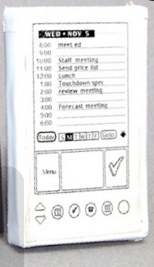
\includegraphics{palmpilot.png}
\caption{پیش نمونه پالم پایلود}
\end{figure}

من فقط میتوانم عکس العمل دیگران را هنگامی که هاوکینز آن تکه چوب را از
جیب خود بیرون می‌آورد و آنرا همانند یک کامپیوتر فعال میفشرد تصور کنم.
آنها فکر میکردند که او دیوانه شده است. اما نه او بسیار باهوش بود. آن تکه
چوب به همراه دکمه‌های پرینت‌شده هاوکینز را به این نتیجه رساند که او راه
درستی را آمده است. او برای اولین و مهمترین سوال پاسخی یافته بود: «اگه من
یک پایلوت داشتم، آیا آنرا با خود حمل کرده و از \textbf{آن چیز} استفاده
میکردم؟» و جواب قطعا «بله» بود و او میدانست که \textbf{چیز} \emph{درست}
را یافته است. اکنون او می‌توانست روی سوالات بعدی تمرکز کند مانند: آیا
می‌توانم آنرا کوچک درست کنیم؟ ساخت آن چقدر هزینه خواهد برد؟ عمر باتری‌ها
چقدر خواهد بود؟ اکنون زمان ساخت یک «نمونه اولیه مناسب» رسیده بود.

پالم پایلوت تنها موفق نبود بکله یک موفقیت بسیار بزرگ با تاثیر عظیم بود.
پایلوت جد تمامی تلفن‌های هوشمند امروزی است. این محصول تنها از تکه چوبی
شروع شد همانند پینوکیو.

\section{وانمود کنید قبل از اینکه
بسازید}\label{ux648ux627ux646ux645ux648ux62f-ux6a9ux646ux6ccux62f-ux642ux628ux644-ux627ux632-ux627ux6ccux646ux6a9ux647-ux628ux633ux627ux632ux6ccux62f}

داستان‌های تبدیل گفتار به متن و پالم پایلوت چیزهای مشترک بسیاری دراند.

\begin{quote}
هر دو تیم شک‌های زیادی درباره سودمندی و قابلیت استفاده و پذیرش ایده خود
داشتند. هر دو ایده جالب بود. درست به نظر میرسیدند. مساله‌ای را حل
می‌کردند. اما آیا آنها یک \textbf{چیز} \emph{درست} بودند؟ آیا مردم واقعا
از آنها استفاده می‌کردند؟ جف هاوکینز حتی سالهای زیادی را برای توسعه
محصول (گریدپد) که «پدیده اعجاز انگیز مهندسی اما یک شکست تجاری بود»، از
دست داده بود(یک \textbf{چیز} \emph{غلط}) و تصمیم داشت که «این اشتباه را
دوباره تکرار نکند».
\end{quote}

\begin{quote}
بخاطر شکشان هر دو تیم میخواستند کاربردپذیری و سودمندی ایده‌هایشان را با
ساختن یک نمونه اولیه آزمایش کنند. همچنین قبل از اینکه شروع به توسعه
محصول کنند، بازخوردهای \emph{استفاده واقعی از محصول}(بجای \emph{نظرات در
مورد محصول}) را جمع آوری کنند.
\end{quote}

\begin{quote}
در هر دو آزمایش اما توسعه حتی یک «نمونه اولیه مناسب»(نسخه خام ولی
عملیاتی محصول نهایی) زمان بسیار و سرمایه‌گذاری قابل توجهی برای تحقیق و
توسعه نیاز داشت.
\end{quote}

\begin{quote}
راه حل آنها برای مشکل «نمونه اولیه مناسب» این بود که \emph{تظاهر} به
داشتن یک چنین نمونه اولیه‌ای کنند. در مثال تبدیل گفتار به متن، سخت افزار
و نرم‌افزار با کمی حیله گری جایگزین شده بود و در پالم پایلوت با قوه تخیل
هاوکینز جایگزین شده بود. \emph{وانمود کنید قبل از اینکه آنرا بسازید}
\end{quote}

به نظر من این دو داستان بخاطر تفاوت بسیار از آنچه افراد و کمپانی‌ها
بصورت معمول در پیگیری ایده‌های نوشان انجام می‌دهند قابل توجه و موثر
بودند. بیشتر مردم عاشق ایده‌ی شان می‌شوند(آن \textbf{چیز} آنها) و فرض
می‌کنند که آن \textbf{چیز} موفق خواهد بود(آن \textbf{چیز} \emph{درست})
پس شروع به ساختن آن می‌کنند. آنها پیش از موعد شروع به تمرکز و
سرمایه‌گذاری روی چیزهای غلط در زمان غلط می‌کنند. بصورت دقیق‌تر، آنها
بیشتر از نیاز و پیش از موعد روی توسعه اولین نسخه محصول خود که دارای
ویژگی‌های زیاد، کارکردهای بیش از حد و «رنگ و لعاب» بیش از حد نیاز است،
سرمایه‌گذاری می‌کنند. آنها پیش‌فرضشان بر این است که مردم آنرا خواهند
خواست. در بسیاری از موارد، این پیش‌فرض ها و فرضیات هم غلط و هم پر هزینه
از کار در می آیند.

\section{پیش‌نمونه سازی: کلمه بوجود
آمد}\label{ux67eux6ccux634ux646ux645ux648ux646ux647-ux633ux627ux632ux6cc-ux6a9ux644ux645ux647-ux628ux648ux62cux648ux62f-ux622ux645ux62f}

من هرچه بیشتر در مورد تبدیل آزمایش متن به گفتار و پالم پایلوت فکر
میکردم، بیشتر قانع می‌شدم که کاری که آن تیم‌ها انجام دادند نه تنها
هوشمندانه بودند بلکه این یک مرحله ضروری در روند توسعه یک محصول جدید و
خلاقانه است. مرحله‌ای که اکثر افراد آنرا از قلم انداخته و اغلب منجر یه
پرداخت هزینه زیادی بخاطر این نادیده گرفتن می شوند.

در طول چند ماه، من این دو داستان را با گروه قابل توجهی از دوستان،
همکاران، کارآفرینان، سرمایه‌گذاران پر ریسک، مهندسان و مدیران محصول به
اشتراک گذاشتم. با تعجب، هیچکدام از آنها این مثال‌ها را قبلا نشنیده
بودند. همه آنها، اما تحت تاثیر راه حل هوشمندانه «وانمود کنید قبل از
اینکه آنرا بسازید» قرار گرفته بودند و برخی از آنها حتی به پیشانی خود
زدند و چیزهایی شبیه «کاش من به همچنین روشی عمل میکردم قبل از اینکه
سال‌ها و میلیون‌ها دلار را روی ایده آخرم از دست میدادم.»

من پیبردم که بصورت اتفاقی به موضوع مهم و ارزشمندی با اینکه جدید یا بکر
نبود، برخورده‌ام که مشهور نبوده و از آن بصورت گسترده استفاده نمی‌شود.
اما این موضوع اسمی نداشت که آنرا توصیف کند و من فکر کردم که این موضوع
برای شناخته شدن، مورد بررسی قرار گرفتن و استفاده نیاز به نامی دارد. پس
من شروع به فکر در مورد اسم برای این موضوع کردم(توجه: من در زمان شروع فکر
در این مورد پیش‌نمونه سازی من در مورد \emph{ماشین استارت آپ ناب} که توسط
اریک ریس و \emph{محصول حداقل مادنی} اطلاعاتی نداشتم. بیشتر در مورد رابطه
بین پیش‌نمونه سازی و محصول حداقلی ماندنی در بعد آورده می‌شود).

از آنجایی که نقطه اصلی و کلیدی هر دو مثال \emph{تظاهر}بود (کارمندان آی
بی ام تظاهر به ساختن ماشین تبدیل گفتار به متن کردند و جف هاوکینز تظاهر
به داشتن پالم پایلوت در جیب لباس خود می‌کرد) اولین کلمه‌ای که به ذهن
میرسید\_‌نمونه اولیه متظاهر\_ است ایش! تلاش دوم من برای پیدا کردن نام
حتی بدتر بود. از آنجایی که ایده‌اصلی تست سریع ایده \emph{قبل} از گذاشتن
سرمایه کافی برای نمونه اولیه مناسب است، من به کلمه \emph{پیش نمونه اولیه
سازی} رسیدم، ایش ایش! خوشبختانه این دو کلمه بد نطفه یک کلمه بهتر را
ایجاد کردند. با حذف برخی از کلمات، من به \emph{پیش‌نمونه سازی} رسیدم.
خیلی خوب. چیزهایی که در روند پیش‌نمونه سازی تولید می‌شوند(مانند قطعه چوب
هاوکینز) پیش‌نمونه گفته می‌شوند.

من از اصطلاحات پیش‌نمونه‌سازی و پیش‌نمونه خوشم می‌آید اما آیا من اولین
نفری هستم که از این کلمه استفاده می‌کنم؟ ممکن است تا الان کسی از این
اصطلاحات استفاده کرده باشد و «حقوقی» را برای استفاده از آن و معنای آن در
نظر گرفته باشد. من به گوگل رفتم و کلمه «پیش‌نمونه سازی» را جستجو کردم.
گوگل در پاسخ گفت «آیا شما نمونه اولیه سازی را میخواستید؟» که باعث
خوشحالی من شد. موتور جستجو فرض میکرد که من اشتباه نوشته باشم و نتایج
مربوطه به نمونه اولیه را نشان میداد که یک نشانه خوب بود. وقتی من بر
اینکه منظورم نمونه اولیه سازی نبوده است تاکید کردم تا گوگل نتایج
پیش‌نمونه سازی را به من نشان بدهد گوگل صفحات اندکی را که مردم در آن
نمونه اولیه را اشتباه نوشته بودند را آورد. جستجوی پیش‌نمونه نیز نتایج
مشابهی داشت. افق روشن در مقابل بود. من اتفاقی کلمه جدیدی پیدا کرده بودم
که کسی هنوز از آن استفاده نکرده بود.

حتی دامنه‌های اینترنتی مربوط به آنها نیز آزاد بود. اولین عکس العمل غریضی
من این بود که با استفاده از کردیت کارتم تمامی آنها را بخرم، اما من با
این کار من پیغام اصلی پیش‌نمونه سازی را نقض خواهم کرد و قبل از اینکه این
موضوع ارزش سرمایه گذاری کردن داشته باشد روی آن سرمایه گذاری کرده‌ام.
باوجود اینکه خریدن دامنه تنها چند دلار هزینه خواهد داشت، اصول ارجحیت
داشت. من فکر میکردم پیش‌نمونه سازی و پیش‌نمونه‌ها توصیف کننده یک مفهوم
عظیم بودند اما آیا مردم نیز چنین احساسی دارند؟ من مجبور به ساختن
پیش‌نمونه پیش‌نمونه سازی بودم.

خوشبختانه، کار من در گوگل شامل صحبت کردن با افرادی زیادی در مورد خلاقیت
و ارائه این موضوع به مشتریان و همکاران بود. پس من در کنار توضیح دو مثال
تبدیل متن به گفتار و پالم پایلوت شروع به استفاده از کلمه پیش‌نمونه و
پیش‌نمونه سازی در تمامی ارائه‌ها، ملاقات‌ها و بحث‌هایم کردم. در یک حالت
افراد بازخورد بسیار مثبتی نسبت به مفهوم و کلمات انتخابی داشتند. آنها
مثال‌هایی از پیش‌نمونه‌هایشان را برای من اراسلا می‌کردند و نظر من را در
مورد نحوه پیش‌نمونه سازی ایده‌هایشان می‌پرسیدند. حتی آنها با همکاران و
مدیران خود برای ساختن پیش‌نمونه‌ها چانه می‌زدند. به نظر میرسید که من در
مسیر درستی بودم.

یک روز من ایمیلی از مدیری یکی از بزرگترین شرکت‌های تبلیغاتی که در ارائه
من در مورد نوآوری شرکت داشت دریافت کردم. او از من بخاطر برگزاری این
ارائه تشکر کرد و گفت که او و تیمش از مفهوم پیش‌نمونه سازی را دوست دارند
و اینکه «\ldots{} کلمه پیش‌نمونه سازی اکنون وارد دایره لغات شرکت آنها
شده است.»

آن روز من شواهد کافی مبنی بر اینکه پیش‌نمونه سازی و پیش‌نمونه کلمات
درستی برای آن مفهوم هستند. من آنروز مطمئن شدم که سرمایه گذاری چند دلار
بیشتر برای خرید دامنه مرتبط سرمایه گذاری کنم.

\chapter{حتما شکست خواهد خورد}
شما الان یک ایده خام از آنچه پیش‌نمونه سازی درباره آن صحبت می‌کند دارید
و ما مثال‌های بیشتری را در فصل‌های آتی مطرح خواهیم کرد. اما قبل از این
مثال‌ها من قصد دارم اندکی زمان برای توضیح چرایی اهمیت زیاد پیش‌نمونه
سازی برای تمام ایده‌هایتان اختصاص می‌دهم.

آیا شما آمارهای ناامید کننده از بخش قبل را به یاد می‌آوردی

\begin{itemize}

\item
  ۹۰ درصد تمامی نرم‌افزارهای موبایل هیچ درآمدی ندارند.
\item
  هر چهار استارت‌آپ از پنج استارت آپ سرمایه سرمایه‌گذاران خود را از دست
  می‌دهند.
\item
  ۸۰ درصد رستوران‌های جدید در سال اول شکست می‌خورند.
\end{itemize}

اعداد دقیق ممکن است متفاوت باشد، اما پیغام این اعداد روشن است. با بیان
ساده اکثر \textbf{چیز}ها-که شام ایده‌ی شما می‌شود- تقدیرشان شکست است.
اکثر \textbf{چیزها} شکست می‌خورند بخاطر اینکه آنها \textbf{چیز}
\emph{غلط} هستند یعنی ایده‌هایی که ابتدا بصورت تئوری جالب به نظر
می‌رسیدند اما هنگامی که توسعه یافتند مشخص گردید که حتی آنها برخلاف آنچه
در ابتدا به نظر می‌رسد اندکی جالب، ترغیب کننده و یا کاربردی نبوده اند.

پیش‌نمونه سازی قدرت تبدیل یک \textbf{چیز} \emph{غلط} را به یک
\textbf{چیز} \emph{درست} ندارد و هیچ روش دیگری این امکان را نخواهد داشت.
اما پیش‌نمونه سازی امکان تشخیص \textbf{چیز}های \emph{غلط} بصورت سریع و
ارزان فراهم می‌کند پس شما می‌توانید \textbf{چیز}های جدید را امتحان
کنید(یا حتی نسخه‌های تغییر یافته \textbf{چیز}های فعلی) تا اینکه شما آن
\textbf{چیز} \emph{درست} گریزپا را بیابید.

از آنجایی که شکست دشمن ماست، و شناخت دشمن مهم است پس بیاید به شکست نگاه
دقیق‌تری داشته باشیم.

\section{قانون
شکست}\label{ux642ux627ux646ux648ux646-ux634ux6a9ux633ux62a}

شواهد در مورد وجود اتفاقات عجیب و غریب به ضرر \textbf{چیز}های جدید
اینقدر زیاد و قابل اعتماد است که می‌توانن قانونی برای آن اعلام کرد:

\textbf{قانون شکست}

اکثر \textbf{چیز}های جدید شکست می‌خورند، فارغ از اینکه چقدر بی نقص اجرا
شده باشند.

در این قانون کلمه «اکثر» اشاره به درصد بسیار زیاد ناامید کننده (معمولا
70-80-90 درصد) دارد و \textbf{چیز}ها تقریبا به هر چیزی که شما فکرش را
بکنید اطلاق می‌شود: استارت‌آپ‌ها، رستوران‌ها، فیلم‌ها، کتاب‌ها،
نوشابه‌ها، سریال تلویزیونی و غیره. و آن \textbf{چیز} شما در یکی از این
دسته‌های قرار گرفته و قطعا دچار همان بدبیاری‌هایی می‌شود که مابقی
\textbf{چیز}های دیگر دچار می‌شوند.

من هم اکنون شکایت‌های شما را مبنی برا اینکه «خب این قانون چگونه به ما
کمک خواهد کرد؟ این قانون به ما می‌گوید ما به احتمال زیاد شکست می‌خوریم
حتی اگر ما بسیار خوب روی \textbf{چیز}مان کار کرده باشیم. این قانون تنها
به ما بدبیاری می‌دهد و ما را پا در هوا نگه می‌دارد. تنها کاری که این
قانون انجام می‌دهد روحیه ما را پایین آورده و انیزه ما را می‌کشد.»

در ظاهر این حرف درست است و قانون شکست به نظر کمک کننده نمی‌رسد. وقتی
بصورت دقیق صحبت کنیم این قانون حتی یک قانون دقیق نیست. شما می‌توانید
نیوتن را هنگامی که در حال مشاهده جاذبه بود تصور کنید که می‌گوید:
«احتمالا بیشتر اجسامی که رها می‌شوند سقوط می‌کنند؟» اما به دست آوردن این
قانون به نسبت آسان است. او در حال بررسی و مشاهده یک قانون تغییر ناپذیر و
عمومی طبیعی بود. اما در طرف دیگر موفقیت بازار یک محصول مرتبط با رفتار
انسانی است که بسیار متغیر، بی ثبات و (و در اغلب موارد) غیر منطقی است. در
این موضوع، فرموله سازی احتمالی قانون شکست بهترین چیزی است که به دست
می‌آید.

من باور دارم با اینکه \emph{قانون شکست} فاصله زیادی تا کاملا دقیق بودن
دارد، اما از اهمیت زیادی هم برخوردار است. اگر شما این درستی این قانون را
قبول کرده و یا حتی در اکثر اوقات آنرا بپذیرید، و بدانید که خود شما یا آن
\textbf{چیز} شما از این قاعده مستثنی نیستند، نظر شما از «بیایید آن
\textbf{چیز} را انجام دهیم! بیایید آن \textbf{چیز} را بسازیم» به نظر
محتاطانه «بیایید آن \textbf{چیز} را بیازماییم. بیایید پیش‌نمونه آن
\textbf{چیز} را بسازیم» تغییر می‌کند.

من میدانم که «آنرا انجام دهیم» بسیار حذاب و قهرمانانه است. «با مساله
گلاویز شدن»، «شرط بندی زمین‌ها» و «بادبان‌ها رو بکشید» سرآغاز افسانه‌های
بسیاری بودند اما ابتدای شروع شکست‌های فاجعه انگیز نی هستند.

با توجه به آنچه گفته شد، ممکن است وقت‌هایی باشد که شما بخواهید به
اتفاقات بد بی‌توجه باشید و تنها بخواهید بدون در نظر گرفتن نتیجه روی آن
\textbf{چیز} خود فعالیت کنید. من به هیچ وجه شما را از این روش دلسرد
نمی‌کنم. لااقل به ندرت در زندگی‌مان، ما بایستی ریسک‌های بزرگ کرده و تنها
برای رسیدن به آن \textbf{چیز} به پیش برانیم. زمان‌هایی خواهد بود که شما
ساختن یک \textbf{چیز} خاص برای شما مهم‌تر از داشتن یک \textbf{چیز}
\emph{درست} است. ار شما در این وضعیت هستید، لبخندی به \emph{قانون شکست}
بزنید، احتیاط را کنار بگذارید و این کتاب را در زباله بیاندازید و با تمام
قلب روح خود روی آن \textbf{چیز} کار کنید. خدایارتان باشد! من طرف شما
هستم و آرزو میکنم موفق شوید.

اما اگر از سوی دیگر، شما در موقعیتی هستید که ۱۰۰ درصد به یک \textbf{چیز}
خاص پایبند نیستید، بیشینه کردن شانس موفقیت بسیار حساس است. به
\emph{قانون شکست} احترام لازم را بگذارید زیرا \ldots{}

\section{\ldots{} شکست یکی از انتخاب‌ها
نیست}\label{ux634ux6a9ux633ux62a-ux6ccux6a9ux6cc-ux627ux632-ux627ux646ux62aux62eux627ux628ux647ux627-ux646ux6ccux633ux62a}

این درست است. برای هر \textbf{چیز}، شکست یکی از انتخاب‌ها نیست بلکه
محتمل‌ترین خروجی است.

ما نمی‌توانیم از \emph{قانون شکست} فرار کنیم. ما نمی‌توانیم شانس
\textbf{چیز}های جدید را تغییر دهیم.

اما آنچه ما می‌توانیم انجام دهیم این است که از \emph{قانون شکست} به نفع
خودمان استفاده کنیم همانگونه که حسابداران از قوانین مالیاتی استفاده
می‌کنند و لیدی گاگا از پاپاراتزی‌ها.

چگونه می‌توانیم این را انجام دهیم؟

ما شکست را دعوت می‌کنیم، ما به دنبال شکست می‌رویم، ما آنرا شکار می‌کینم
تا چهره کریه خود را در اولین فرصت ممکن به ما نشان بدهد تا ما بدانیم که
راه غلطی را طی می‌کنیم. پس بتوانیم در زودترین موقع تغییرات لازم را انجام
دهیم.

ما چندین طعمه در شکل پیش‌نمونه جعل می‌کنیم. بعضی وقت‌ها آنها شبیه یا بوی
آن \textbf{چیز} ما را می‌دهد. چیزی که ما بتوانیم با کمک آن \emph{دیو
شکست} را مجبور به نشان دادن سر کریه‌ش بکنیم. ما به در غار تاریک و
نم‌ناکی که دیو در آن ساکن است می‌رویم. آنگاه طعمه پیش‌نمونه خود را در
ورودی این غار گذاشته تا ببینیم که دیو به طعمه نزدیک می‌شود که ما بتوانیم
بوی بد تنفسش را بشنویم و بتوانیم نگاه کوتاهی به به دهان بی‌رحمش و چشمان
کوچکش بیاندازیم. آنقدر نزدیک که مطمئن شویم که دیو واقعی است. آنگاه طعمه
ارزان قیمت خود را به عنوان قربانی به دیو تقدیم کرده و در جهت مخالف فرار
کنیم. قبل از اینکه دیو بتوانی دندان‌های تیزش را در گوشت ما فرو کرده و ما
را به درون غار خود کشیده و از ما جشنی برپا کند.

\chapter{پیش‌نمونه‌اش را بسازید}
مقدمه‌چینی، توجیه، توضیح و تعریف کافی است. وقت آن است که به خوراک اصلی
این کتاب برسیم - روندد واقعی تولید و تست یک پیش‌نمونه.

در ابتدا، انواع اولیه پیش‌نمونه سازی را برای شما معرفی می‌کنم و سپس به
راه‌های تست آنها نگاهی انداخته و در نهایت تمام آنچه را آموخته‌ایم را در
چند مثال کامل تجمیع می‌کنم.

\section{تکنیک‌های درهم برهم پیش‌نمونه
سازی}\label{ux62aux6a9ux646ux6ccux6a9ux647ux627ux6cc-ux62fux631ux647ux645-ux628ux631ux647ux645-ux67eux6ccux634ux646ux645ux648ux646ux647-ux633ux627ux632ux6cc}

روزی اگر این کتاب مبدل به یک \textbf{چیز} \emph{درست} شد، من سرمایه
زمانی بیشتری برای تولید ساختار سلسله مراتبی روش‌های پیش‌نمونه سازی میکنم
که بصورت کامل با ساختار درست و بصورت رسمی این تکنیک‌ها را ارائه می‌دهد.
در آن زمان به هر روش یک نام فانتزی داده، سناریو ایده‌آل استفاده از آن را
ارائه کرده و مثال‌های بسیاری میزنم. اما از آنجایی که خود این کتاب هنوز
یک پیش‌نمونه است، چیزی شما خواهید دید یک لیست درهم برهم از روش‌ها به
همراه توصیف خام اینکه هر روش کی و چگونه مورد استفاده قرار می‌گیرد.

لیست خلاصه این روش‌ها که قرار است در مورد آنها صحبت کنیم از قرار زیر
است:

\begin{itemize}
\item
  \textbf{ترک مکانیکی} - انسان‌ها را جایگزین کامپیوترها یا ماشینهای
  پیچیده و گران قیمت کنید.
\item
  \textbf{پینوکیو} - نسخه غیر عملیاتی و «مرده» محصول خود را بسازید.
\item
  \textbf{کمینه محصول پذیرفتنی(یا محصول کوچک شده)}: یک محصول عملیاتی آن
  \textbf{چیز} رابسازید، اما آنقدر آنرا کوچک کنید که فقط ویژگی‌‌های
  اساسی باقی بماند.
\item
  \textbf{استانی} - قبل از اینکه در کل جهان محصول خود را ارائه کنید،
  آنرا روی مجموعه کوچکی تست کنید.
\item
  \textbf{در جعلی} - یک «ورودی» جعلی برای محصولی که اصلا وجود خارجی
  ندارد بسازید.
\item
  \textbf{وانمود کنید که دارید} - قبل از سرمایه گذاری برای خرید هر چیزی
  که برای \textbf{چیز}تان به آن نیاز دارید، آنرا قرض گرفته یا اجاره
  کنید.
\item
  \textbf{لیبل گذاری مجدد} برچسب جدید روی محصول فعلی که شبیه آن چیزی است
  که شما میخواهید آنرا تولید کنید بگذارید.
\end{itemize}

در استفاده، سوء استفاده، استفاده غلط یا استفاده نابجا از هریک از این
تکنیک‌ها آزاد هستید.آنها را ترکیب، پالایش، باز تعریف نموده و آنها را به
دانش شخصی خود اضافه کنید. اگر شما یک روش جالب پیش‌نمونه سازی پیدا کرده و
یا پیشنهادی در این مورد دارید حتما من را در جریان قرار دهید. آنرا توصیف
نموده و به آن نامی بدهید و ممکن است من آنرا در نسخه بعدی کتاب بگنجانم یا
در وبلاگم آنرا ارائه دهم.

حالا نوبت توضیح بیشتر در مورد هر تکنیک است.

\section{ترک
میکانیکی}\label{ux62aux631ux6a9-ux645ux6ccux6a9ux627ux646ux6ccux6a9ux6cc}

این تکنیک پیش‌نمونه سازی نامش را از یک «ماشین» بازی شطرنج به همین نام
قرض گرفته است. این ماشین در انتهای قرن ۱۸ میلادی در سراسر دنیا به نمایش
گذاشته شد. به مردم قبولانده می‌شد که «ترک» یک ابداع مکانیکی است که
برنامه ریزی شده تا شطرنج بازی کند. در واقع، درون جعبه یک شطرنج باز با
استعداد و کوچک قرار داشت که با استفاده از دسته‌های ماشین شطرنج بازی
می‌کرد.

\begin{figure}[htbp]
\centering
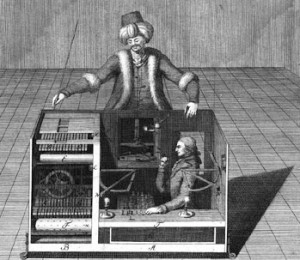
\includegraphics{mechanicaltork.png}
\caption{ترک میکانیکی}
\end{figure}

پیش‌نمونه‌های ترک میکانیکی برای موقعیت‌هایی که می‌توان انسان را بصورت
مخفی جایگزین تکنولوژی‌های پرهزینه، پیچیده یا نیازمند توسعه در آینده کرد
ایده‌آل است. آزمایش تبدیل متن به گفتار آی بی ام نمونه به نقصی از این روش
است. توسعه یک موتور تبدیل متن به گفتار سالهای زمان و سرمایه گذاریی عظیمی
نیاز داشت اما یک تایپیست انسانی که در اتاق کناری مخفی شده بود به راحتی
این کارایی پیچیده را شبیه سازی کرد. همانند شطرنج باز درون ترک میکانیکی.

\section{پینوکیو}\label{ux67eux6ccux646ux648ux6a9ux6ccux648}

این روش پیش نمونه سازی از بلوک چوبی پالم پایلوت جف هاوکین بدست آمده است
و نامش را از عروسک چوبی گرفته است که بعد از ملاقات با پری آبی تبدیل به
یک پسر واقعی شد.

پیش نمونه پینوکیو برای حالاتی که سایز، شکل، وزن، حمل پذیری و غیره مهم
است بهترین تناسب را دارد. همچنین در جاهایی که خیال‌پردازی فرد برای پر
کردن جاهای خالی کافی است مناسب است. این دقیقا همان کاری است که جف هاوکین
تظاهر می‌کرد که بلوک چوبی او قابلیت زمان‌بندی کارهایش، ذخیره شماره تلفن
و یادداشت برداری را دارد.

\section{کمینه محصول پذیرفتنی(یا محصول کوچک
شده)}\label{ux6a9ux645ux6ccux646ux647-ux645ux62dux635ux648ux644-ux67eux630ux6ccux631ux641ux62aux646ux6ccux6ccux627-ux645ux62dux635ux648ux644-ux6a9ux648ux686ux6a9-ux634ux62fux647}

کلمه کمینه محصول پذیرفتی توسط اریک ریس معرفی و به شهرت رسید. اریک خالق
حرکت استارتاب ناب بوده و یکی از قهرمان‌های شخصی من است.

همانطور که این نام پیشنهاد می‌کند، این تکنیک شامل ساختن یک پیش‌نمونه‌
است که کاری را انجام می‌دهد(محصول واقعی). اما ویژگی‌ها و کارایی‌ها تا
رسیدن به حداقل حذف شده اند. این کار به منظور «جمع آوری حداکثر اطلاعات
اعتبارسنجی شده از مشتریان با حداقل تلاش» است.

از آنجایی که در کمینه محصول نیازمند یک ویژگی و کارایی اولیه هستیم این
روش پیش‌نمونه‌سازی کار بیشتری نسبت به روش‌های پینوکیو و ترک مکانیکی
می‌برد. اما این محصول کمینه بسیار سریع‌تر از محصول اصلی توسعه می‌یابد
زیرا از شر تمام ویژگی‌های غیر حیاتی راحت شده است. یک محصول کمینه برای
نرم افزار دفتر خاطرات خانودگی تنها از ورودی متن و شاید در کنار یک عکس
پشتیبانی می‌کند و از فونت‌های گوناگون برای متن، ویدئو یا اشتراک
گذاری‌های متفاوت را پشتیبانی نمی‌کند. این ویژگی ممکن است خوب بوده و حتی
برای موفقیت محصول نهایی مورد نیاز باشند اما بایستی پس از بررسی اولیه این
موضوع که دفتر خاطرات خانوادگی یک \textbf{چیز} \emph{درست} است یا نه،
اضافه گردد.

\begin{quote}
همانطور که قبلا هم اشاره کردم، من در مورد محصول کمینه ماشین استارتاپ ناب
چند ماه بعد از اینکه صحبت در مورد پیش‌نمونه سازی و ساختن آنها را شروع
کرده بودم شنیدم.در یک کارگاه، من در مورد این محصول کوچک شده(نامی که من
در آن موقع از آن استفاده می‌کردم) یک نرم افزار موبایل صحبت میکردم و کسی
از حضار به من گفت که: «این چه تفاوتی با مفهوم محصول کمینه پذیرفتنی اریک
ریس دارد؟» من آن موقع جواب قابل قبولی نداشتم. اما بعد از یادگرفتن در
مورد محصول کمینه و کارهای اریک ریس متوجه شدم که محصول کمینه و پیش‌نمونه
سازی(به همراه روش ماشین استارتاپ ناب) قصد دارند تا به کارآفرینان،
سازندگان و مخترعان کمک کنند که یک اشتباه اساسی را انجام ندهند: سرمایه
گذاری مالی و زمانی زیادی برای ساختن محصولاتی است که بازاری نداشته یا
بازار قابل قبولی که ارزش این سرمایه گذاری را داشته باشند ندارد.

اگر شما به این کتاب علاقه مند هستید، شما باید کتاب استارت آپ ناب اریک
ریس را خریده و بخوانید. این یک کتاب عالی است که همه بهتر است آنرا
بخوانند چه آنهایی که در یک استارت‌آپ مشغولند و چه آنهایی که در شرکت‌های
بزرگ کار می‌کنند.
\end{quote}

\section{محلی}\label{ux645ux62dux644ux6cc}

در بسیاری از موارد، هزینه اصلی تولید یک محصول، توسعه ویژگی‌های اولیه
نیست بلکه افزایش کارایی آن برای پشتیبانی از حجم زیادی کاربر است. یک
پیش‌نمونه محلی ویژگی‌های اصلی محصول نهایی را فراهم آورده و محدوده (و
کارایی) خود را به زیر مجموعه کوچکی از بازار هدف نهایی محدود می‌کند. مثل
همیشه بگذارید با مثال این مورد را توضیح دهم.

بیایید فرض کنیم که سندرا ایده‌ای برای یک نرم‌افزار موبایل داشته که به
افراد کمک می‌کند که رستوران‌هایی که غذای ارگانیک ارائه میکنند را پیدا
کنند. بگذارید \textbf{چیز} سندرا را \emph{دستیار غذای ارگانیک} بنامیم.

یکی از پر هزینه ترین و زمان بر ترین بخش‌های این نرم افزار تولید و
نگهداری پایگاه‌داده ای از رستوران‌های سطح کشور است که تنها غذای ارگانیک
ارائه میکنند. ممکن است در کل کشور هزارن رستوارن از این نوع وجود داشته
باشد و جمع آوری تمام آنها و نوشتن برنامه‌ای که آنها را به روز نگهدارد
کار زیادی برای سندار خواهد داشت. کار زیادی که در صورتی که ایده
\emph{دستیار غذای ارگانیک} یک \textbf{چیز} \emph{درست} نباشد غیر لازم
بوده و به هدر رفته است.

یک نمونه محلی ممکنه به صورت زیر توسعه یابد: سندرا بایستی خود را به شهر
یا بخش خاصی(بصورت ایده آل جایی که خود زندگی می‌کند) خود را محدود کند. از
آنجایی که ممکن است تنها تعداد محدودی رستوران ارگانیک در محدوده‌ای که
انتخاب کرده است باشد، توسعه نرم‌افزار بسیار ساده خواهد شد. سندرا میتواند
نام و موقعیت رستوران‌ها را در برنامه \emph{هارد کد} کند بجای اینکه از یک
پایگاه داده مرکزی آنها را بازیابی نموده و نزدیک‌ترین‌ها را به نمایش
بگذارد.

علاوه بر اینکه روش محلی روند توسعه نرم‌افزار ساده سازی کرده و به آن شتاب
داده است، این روش زمان و کار مورد نیاز برای بازاریابی و تست بازار را نیز
کاهش داده است. بجای تبلیغ نرم‌افزار در سطح کشور او می‌تواند روی بخش
کوچک‌تری متمرکز شده و پول بسیاری را ذخیره نموده و یادبگیرد که آیا
نرم‌افزار او یک \textbf{چیز} \emph{درست} است یا خیر؟

\section{پیش‌نمونه در
جعلی}\label{ux67eux6ccux634ux646ux645ux648ux646ux647-ux62fux631-ux62cux639ux644ux6cc}

اسم این تکنیک از ارائه‌ی جس لی(یکی از بنیانگذاران و مدیر محصولات برند
پلیور) گرفته شده است. جس بابت این اسم عالی ممنون!

با پیش‌نمونه در جعلی تنها نیاز ساختن یک «مدخل» یا «ورودی» برای یک
محصول(یا ویژگی) بالقوه است. اصلا نیازی به وجود محصول(یا ویژگی) نیست. جس
اینگونه می‌گوید که «در یک محصول تحت وب، بدین معناست که شما
\textbf{وانمود} کرده که ویژگی وجود دارد و شما بررسی می‌کنید که آیا کسی
روی آن کلیک خواهد کرد»

پیش‌نمونه در جعلی برای حالاتی که قرار میزان علاقه به آن \textbf{چیز}
سنجیده شود مناسب است.

در اینترنت یک در جعلی میتواند به عنوان یک لینک، یک دکمه روی صفحه وب یا
یک تبلیغ تحت وب برای \textbf{چیز} شما باشد.

فرض کنید سندی به فکر نوشتن یک کتاب در مورد \emph{مشاهده سنجاب‌ها}(یک از
انواع سرگرمی عجیب مشاهده پرندگان) است. قبل از اینکه او ماه‌ها زمان
ارزشمند خود را روی کتاب مشاهده‌ی سنجاب‌ها «یک مشاهدگر سنجاب کارکشته»
بگذارد، سندی از پیش‌نمونه در جعلی را بکار می‌برد. به منظور درک علاقه‌ی
افراد به این موضوع او یک تبلیغ تحت وب به چنین مضمونی درست می‌کند

\begin{quote}
یک مشاهده گر سنجاب کارکشته. تنها کتاب مشتاقان سنجاب. تنها ۹.۹۸ دلار.
برای اطلاعات بیشتر اینجا کلید کنید.
\end{quote}

او می‌تواند با استفاده از سرویس تبلیغات گوگل تبلیغ و سایت مرتبط با سنجاب
خود را به افرادی که به دنبال «مشاهده سنجاب» می‌گردند به نمایش بگذارد.

ما همچنین یک مثال کامل‌تر از این روش را در فصل «کنار هم قرار دادن
تکه‌ها» خواهیم داشت. من مطمئن هستم که شما و مابقی مشاهده کنندگان سنجاب
نمی‌توانید تا آن موقع صبر کنید.

\section{وانمود کنید
دارید}\label{ux648ux627ux646ux645ux648ux62f-ux6a9ux646ux6ccux62f-ux62fux627ux631ux6ccux62f}

برخی از \textbf{چیز}ها ممکن است نیاز به سرمایه‌گذاری اولیه بسیاری داشته
باشند در این حالت‌ها،حیاتی است که پیش‌نمونه‌ی ایده شما آن اشیاء گران
قیمت را قرض گرفته یا اجاره کنند.

کسب و کاری که به عنوان مثال نیاز به یک مغازه فیزیکی داشه باشند تا زمانی
که از مناسب بودن ایده خود اطمینان ندارند نباید به یک قرارداد ۵ ساله
اجاره تن در دهند. آنها می‌توانند یک قرار داد سه ماهه یک فضای کوچک
راگرفته یا حتی در حالت بهتر بخشی از مغازه کسی را که خریدارانی مشابه
دارد، اجاره کنند.

ایده شرکت ارائه خدمات قرض ماشین‌های \emph{سبز} که تنها ماشین‌های
الکتریکی را اجاره می‌دهد را بایستی با اجاره یا قرض چند ماشین برقی برای
چند هفته تست کرد بجای اینکه یک مجموعه از آنها را در ابتدا خرید.

اصل مطلب بیان شد. تا زمانی که مطمئن نیستید یک \textbf{چیز} \emph{درست}
را دارید همه چیز را ارزان تمام کنید.

\section{ملاحظات
اخلاقی}\label{ux645ux644ux627ux62dux638ux627ux62a-ux627ux62eux644ux627ux642ux6cc}

برخی از این ایده‌ها از نظر اخلاقی ممکن است شما را در محضوریت قرار دهد
مگر اینکه شما روانپریشی با اختلال شخصیت مرزی باشید. آیا واقعا درست کردن
یک «در جعلی» برای اینکه بسنجیم آیا افراد روی آن کلیک می‌کنند درست است؟

من بسیار در این مورد فکر کرده‌ام و به نتیجه زیر رسیده‌ام:

\textbf{چیز}های \emph{غلط} مسئول هدررفت‌های بزرگ هستند. آنها زمان افراد
زیرکی را که مسئول توسعه آنها هستند را هدر می‌دهند همچنین پول و
سرمایه‌هایی طبیعی را که می‌تواند صرف ساختن چیزهای بهتر و کارا تر شوند.
زمان، هزینه و منابعی که روی \textbf{چیز}های \emph{غلط} سرمایه گذاری
می‌شوند همان زمان، هزینه و منابعی است که از \textbf{چیز}های \emph{درست}
دزدیده می‌شوند.

به تمام محصولاتی که خریده‌اید و تنها یکبار یا دو بار قبل از دورانداختن
یا جایگزین کردن، از آنها استفاده کرده‌اید فکر کنید. به تمام محصولات
فروخته نشده‌ای که از محل دفن زباله سردر می‌آورند فکر کنید.

پیش‌نمونه سازی می‌تواند شما و مشتریان بالقوه شما را از هدر دادن زمان و
پول زیاد روی \textbf{چیز}های \emph{غلط} نجات دهد.

از قضاوت و اخلاقیت خود هنگاهم توسعه و تست پیش‌نمونه‌ها کمک بگیرید و قطعا
شما شب با آرامش خواهید خوابید.

\chapter{‌آنرا تست کنید}
پیش نمونه‌های تنها به یک دلیل ساخته می‌شوند و آن دلیل کمک به ما در تعیین
میزان علاقه و عکس العمل مردم به آن \textbf{چیز} ماست. داده‌های که ما به
کمک پیش‌نموه‌ها جمع آوری می‌کنیم به ما کمک می‌کنند که تعیین کنیم ایده‌ی
ما یک \textbf{چیز} \emph{درست} است یا نه.

تنها راه کارا برای دانستن اینکه یک \textbf{چیز} یک \textbf{چیز}
\emph{درست} است تست کردن آن است.این جمع آوری نه در سرزمین افکار با جمع
آوری ایده‌های انتزاعی و نظرات ذهنی صورت می‌گیرد بلکه در دنیای واقعی با
استفاده از یک پیش‌نمونه‌ی ساخته شده از کاربران واقعی صورت می‌گیرد.

\section{داده‌ها بر نظرات
مقدمند}\label{ux62fux627ux62fux647ux647ux627-ux628ux631-ux646ux638ux631ux627ux62a-ux645ux642ux62fux645ux646ux62f}

در گوگل ما چند باور اصلی داریم و آنها «داده‌ها بر نظرات مقدمند»و «آنرا
به کمک اعداد بیان کن» است.

اما ما به کمک پیش‌نمونه‌هایمان چه نوع داده‌ای باید جمع آوری کنیم؟ و
اینکه آنها را به چه اعدادی «بیان» کنیم؟

تقریبا داشتن یک مجموعه ثابت از معیارها که به تمام \textbf{چیز}ها قابل
اعمال باشد غیر ممکن است. به عنوان مثال موفقیت یک کتاب با تعداد فروش آن
اندازه گیری میشود و یک فیلم با فروش گیشه‌ای اش. اما در طرف دیگر موفقیت
یک سرویس تحت وب مثل گوگل یا جیمیل با تعداد افرادی که اسم نویسی می‌کنند
مشخص نشده بلکه از استفاده‌کنندگانی که بصورت متناوب(استفادکنندگانی که ۷
روز هفته را فعالند) از حسابشان استفاده می‌کنند مشخص می‌شود.

در عینی حالی که مجموعه‌ی کلی از معیارهای موفقیت وجود ندارد، خط مشی‌هایی
وجود داشته که به کمک کمی اصلاح به تمامی \textbf{چیز}ها قابل اعمالند.

از آنجایی که خود این کتاب نسخه پیش‌نمونه کتاب است(به بخش مرتبط با محصول
کمینه قابل قبول مراجعه کنید) در اینجا تنها به معرفی دو معیار اولیه اما
مهم می‌پردازم: \emph{سطح علاقه اولیه} و \emph{سطح علاقه مداوم}

\section{سطح علاقه
اولیه}\label{ux633ux637ux62d-ux639ux644ux627ux642ux647-ux627ux648ux644ux6ccux647}

اولین معیاری که شما باید سعی به جمع اطلاعات در موردش برای همه
\textbf{چیز}ها بپردازید چیزی است که من به آن سطح علاقه اولیه می‌گویم.

این معیار یک نسبت بسیار ساده است:

\begin{quote}
سطح علاقه اولیه = تعداد کارهای انجام شده / تعداد کل پیشنهاد انجام آن کار
\end{quote}

که در آن

\begin{quote}
\emph{تعداد کل پیشنهاد انجام آن کار} نماینده تعداد افرادی است که به آنها
پیشنهاد شده است که کاری با پیش‌نمونه‌ی شما انجام دهند و \emph{تعداد
کارهای انجام شده} نشاندهنده تعداد افرادی است که از پیشنهاد شما استقبال
کرده و کاری انجام داده اند.
\end{quote}

مثل همیشه یک مثل به واضح شدن موضوع کمک خواهد کرد.

آدام یک برهنه گراست و سقوط آزاد کننده آماتور است. او در مورد دو «علاقه»
خود بسیار علاقه مند است و در فکر استعفا دادن از کار خود به عنوان یک
حسابدار(جایی که به او اجازه نمی‌دهند برهنه گرا باشد) و خرید یک هواپیما و
شروع اولین کسب و کار سقوط آزاد برهنه در جهان باشد: \emph{سقوط آزاد
مادرزاد}

آدام قبل از اینکه از کار خود استعفا داده و یک هواپیمای ملخی بخرد، بسیار
خوب خواهد بود(اگر بخواهیم تواضع به خرج دهیم) که بدانیم میزان علاقه به
ایده‌ی او چقدر است. آیا سقوط آزاد برهنه یک \textbf{چیز} \emph{درست} است؟
میدانیم که برهنه‌گراها و سقوط آزاد کنندگان بسیاری وجود دارند. آما چقدر
برهنه‌گرا که دوست دارند سقوط آزاد کنند وجود دارد؟ چقدر سقوط آزد کنندگانی
که دوست دارند تنها و تنها با چترشان بپرند وجود دارد؟ کارهایی که آدام
باید برای مشخص کردن میزان علاقه‌ی انجام بدهد از این قرار است.

فروم‌های آنلاین بسیاری برای برهنه‌گراها و سقوط آزاد دوستان وجود دارد.
فرض می‌کنیم که آدام هم‌اکنون عضو چندتا از آنهاست.

آدام ممکن است پستی به این شکل در فروم برهنه‌گراها بفرستد:

\begin{quote}
برهنه‌گراهای عزیز، من میخواهم یک هواپیما برای سقوط آزاد لختی اجاره کنم.
هزینه ۱۰۰ دلار به ازای هر پرش است. نیازی به تجربه قبلی برای سقوط آزاد
نیست و قول میدهم که یک دشت پر خار فروم نخواهیم آمد. اولین پرش یک ماه
بعد(شنبه ۳۱ می) در سانتا باربارا خواهد بود. برای عضوید به من یک ایمیل
فرستاده که حاوی اسامی و تعداد افرادی که در گروه شما هستند باشد. من پاسخ
شما را با جزئیات لازم خواهم داد. ظرفیت محدود است پس اولویت با آنهایی است
که زودتر درخواست داده‌اند.
\end{quote}

\begin{quote}
آدام
\end{quote}

فرضم کنیم که آدام یک هفته بعد از ارسال پیغامش متوجه می‌شود که ۱۴۹۰ نفر
پستش را خوانده‌اند(این تعداد کل پیشنهاد‌ انجام کار است) و او فقط ۲ ایمیل
در مورد اینکه آنها می‌خواهند شرکت دریافت کرده است(تعداد کارهای انجام
شده).

مقدار سطح علاقه اولیه در این حال ۲/۱۴۹۰ = ۰/۰۰۱۳ است. یا ۰.۱۳ درصد.

خیلی دلگرم کننده نیست، البته خیلی هم تعجب برانگیز نیست زیرا اکثر
افراد(شامل برهنه‌گراها) بصورت طبیعی طرفدار پریدن از یک هواپیما سالم
نیستند. در این نقطه آدام می‌تواند به دو پاسخ دهنده بگوید که او متاسف است
و برنامه سقوط آزاد لخطی به علت عدم علاقه لغو شده است.

اما آدام قبل از کنارگذاشتن ایده‌اش، یک پست مشابه در فروم سقوط آزاد محلی
می‌گذارد. چیزی شبیه این:

\begin{quote}
سقوط آزاد کنندگان عزیز، آیا شما از راه رسم قدیمی پرش خود خسته نشده‌اید؟
برای اینکه اوضاع جالب شود من یک هواپیما برای سقوط آزاد لختی اجاره
کرده‌ام. هزینه ۱۰۰ دلار برای هر پرش است. قول میدهم که یک دشت پر خار فروم
نخواهیم آمد بلکه در یک ساحل لختی فرود خواهیم آمد چه هیجان انگیز. اولین
پرش یک ماه بعد(شنبه ۳۱ می) در سانتا باربارا خواهد بود. برای عضوید به من
یک ایمیل فرستاده که حاوی اسامی و تعداد افرادی که در گروه شما هستند باشد.
من پاسخ شما را با جزئیات لازم خواهم داد. ظرفیت محدود است پس اولویت با
آنهایی است که زودتر درخواست داده‌اند.
\end{quote}

\begin{quote}
آدام
\end{quote}

فرض کنیم که بعد از یک هفته ۸۹۸ سقوط آزاد کننده پست را خوانده‌اند و ۱۱۲
نفر از آنها برای پرش اعلام آمادگی کرده‌اند.

میزان علاقه اولیه در این حالت برابر: ۱۱۲/۸۹۸= ۱۲/۵٪ است که عددی بسیار
بزرگتر است.حالا بیایید صحبت کنیم.

بایک پیش‌نمونه درجعلی و به کمک معیار میزان علاقه اولیه در کمتر از یک
ساعت «کار» دوست سقوط آزاد کننده برهنه‌گرای ما آدام داده‌های با ارزشی جمع
آوری کرده است:

جامعه سقوط آزاد کنندگان بازار هدف بهتری(۱۰۰ برابر بهتر) نسبت به جامعه
برهنگان است.

میزان علاقه اولیه سقوط آزاد کنندگان به نسبت بالاست که این عدد بالای ۱۰٪
به نسبت ۱۰۰۰۰ سقوط آزاد کننده سرتاسر آمریکا به اندازه کافی خوب است که
این ایده را بیشتر مورد بررسی قرار دهیم.

آن درصد از سقوط آزاد کنندگان که ثبت‌نام کرده‌اند بسیار مشتاق بوده و
آماده ثبت نام بودند. این یک سیگنال بسیار قوی در راستای یک \textbf{چیز}
\emph{درست} بودن است.

مقدار علاقه اولیه بسیار قوی و به راحتی قابل تفسیر و مقایسه در برابر یک
مقدار علاقه اولیه دیگر است. در مورد آدام، میزان علاقه اولیه بصورت غیر
مبهمی بیان میدارد که سقوط آزاد کنندگان بازار هدف بهتری از برهنه‌گراها
هستند. اما دانستن آنکه این سطح علاقه اولیه به اندازه کافی خوب است که
ادامه داد یا نه کار سختی است. برای برخی از \textbf{چیز}ها میزان علاقه
اولیه ۱۲/۵ درصدی ممکن است عالی در نظر گرفته شود اما برای برخی دیگر
اینگونه نیست. با توجه داشت در عین حالی که جمع آوری اطلاعات برای محاسبه
میزان علاقه اولیه مهم است، تفسیر آن نیاز به قضاوت و دانش آن حوزه یا
بازار دارد.

اوضاع ایده \emph{سقوط آزاد مادرزاد} خوب به نظر می‌رسد اما میزان علاقه
اولیه یک نشانگر اولیه برای یک \textbf{چیز} \emph{درست} بالقوه است.
بیایید چیزی که آدام باید آنرا پیش‌نمونه‌سازی کند و اندازه بگیرد را بررسی
کنید.

\begin{quote}
\textbf{توجه:} من یک حس غریب در مورد اینکه سقوط آزاد برهنه برخلاف قوانین
هوایی باشد دارم. از آنجایی این کتاب نیز خود یک پیش‌نمونه است، من
تحقیقاتی جامعی در این مورد انجام نداده‌ام. و برای اینکه مطمئن باشم
می‌گویم که من به هیچ‌وجه ایده‌ی سقوط آزاد برهنه را پیشنهاد نکرده و بر آن
صحه نمی‌گذارم پس آنرا در خانه امتحان نکنید. اما اگر کردید، من را برای
انجام این ایده شماتت نکرده و عکس خود را برای من نفرستید.
\end{quote}

\section{سطح علاقه
مداوم}\label{ux633ux637ux62d-ux639ux644ux627ux642ux647-ux645ux62fux627ux648ux645}

برای برخی از \textbf{چیز}ها، موفقیت وابسته به تکرار کسب و کار است(مثلا
یک کتاب یا یک بازی آرکید). میزان خوب سطح علاقه اولیه ممکن است کافی باشد
تا کار را پیش بگیریم. اما \textbf{چیز}های بسیاری هستند که موفقیتشان
وابسته به تکرار خرید، بازدید مجدد، یا استفاده مداوم توسط گروهی از افرادی
است که بصورت اولیه علاقه‌مند به آن \textbf{چیز} بوده‌اند. مخصوصا هنگامی
که راه‌اندازی کسب و کار نیاز به پیش خرید تجهیزات گران‌قیمت یا هزینه
تکرار شونده گران است.

برخلاف میزان علاقه اولیه، سطح علاقه مداوم بجای یک عدد توسط نمودار(جدول)
مبتنی بر زمان به نمایش گذاشته می‌شود. هر مدخل یا نقطه در این نمودار یا
جدول میزان علاقه در یک تاریخ خاص است. ما بهتر است دنبال چه معیاری در
جدول یا گراف سطح علاقه مداوم باشیم؟ آیا علاقه در طول زمان به صفر میل
کرده است؟ آیا یک مقدار کاهش یافته سپس در سطح قابل قبولی به ثبات می‌رسد؟
آیا افزایش می‌یابد؟ در اولین حالت شما احتمالا یک \textbf{چیز} \emph{غلط}
سروکار دارید. در حالت دوم ممکن است اوضاع بهتر یا بدتر شود و نیاز به
بررسی بیشتری دارد. حالت سوم یک نشانه امیدوار کننده است و ممکن شما یک
\textbf{چیز} \emph{درست} داشته باشید.

مثل همیشه توضیح دادن همیشه با استفاده از یک مثلا بسیار ساده‌تر است.
بیایید از جایی که مثال قبل با آدام را رها کرده‌ بودیم را از سر بگیریم و
به سراغ کسب و کار سقوط آزاد برهنه را از سر بگیریم.

در مورد \emph{سقوط آزاد مادرزاد} آدام آدم بی توجه خواهد بود اگر تنها بر
اساس معیار سطح علاقه اولیه از شغلش استعفا داده و یک هواپیمای ملخی بخرد.
حتی اگر بیش از ۱۰٪ تمام سقوط آزاد کنندگان علاقه‌مند به امتحان یک سقوط
برهنه هستند اما اگر آنها برای انجام دوباره اینکار برنگردند این یک کسب و
کار کوتاه خواهد بود.

آدام قبل از گرفتن هر تصمیم(مثل استعفا از شغلش) یا سرمایه(مثل خرید یک
هواپیما ملخی) بزرگ، بایستی سطح علاقه مداوم را اندازه گیری کند.

پیش‌نمونه در جعلی برای تست علاقه اولیه بسیار خوب است اما برای تست سطح
علاقه مداوم به چیزی ملموس‌تر و قابل‌توجه‌تری نیاز است. بیشتر افراد به
باز کردن در جعلی ادامه نخواهند داد. پیش‌نمونه وانمود کردن دارایی در این
مورد کارا خواهد بود.

بجای خرید یک هواپیما، آدام بایستی هواپیما را در موارد مورد نیاز اجاره
کند. اجاره کردن روزانه هواپیما به عنوان یک انتخاب دراز مدت برای
\emph{سقوط آزاد مادرزاد} پرهزینه و غیر عملی است. اما تا زمانی که آدام
متقاعد شود ایده سقوط آزاد برهنه‌ی او موفق خواهد بود خرج کردن چند صد دلار
اضافه برای تست آن بجای خرج ده‌ها هزار دلار سرمایه‌گذاری به امید داشتن یک
\textbf{چیز} \emph{درست} بهتر است. \emph{قانون شکست} را باوجود میزان
علاقه اولیه مثبت به خاطر بیاورید که شانس بر علیه \textbf{چیز} آدام است.

بیایید فرض کنیم که آدام از پروتکل پیش‌نمونه‌سازی پیروی کرده و تبلیغات
خود را در فروم سقوط آزاد هر هفته ادامه داده و در طول دو ماه ۸ پرواز
انجام میدهد: یک پرواز در هر شنبه

دادهای مرتبط با سطح علاقه مداوم برای دو ماه به شرح زیر است

\begin{longtable}[c]{@{}lcrll@{}}
\toprule\addlinespace
شماره پرواز & تعداد ثبت نام & درآمد & هزینه & سود/زیان
\\\addlinespace
\midrule\endhead
۱ & ۲۱ & ۲۱۰دلار & ۲۵۰دلار & -۴۰ دلار
\\\addlinespace
۲ & ۲۰ & ۲۵۰دلار & ۲۵۰دلار & ۰ دلار
\\\addlinespace
۳ & ۲۸ & ۲۸۰دلار & ۲۵۰دلار & ۳۰ دلار
\\\addlinespace
۴ & ۱۷ & ۱۷۰دلار & ۲۵۰دلار & -۸۰ دلار
\\\addlinespace
۵ & ۷ & ۷۰دلار & ۲۵۰دلار & -۱۸۰ دلار
\\\addlinespace
۶ & ۳ & ۳۰دلار & ۲۵۰دلار & -۲۲۰ دلار
\\\addlinespace
۷ & ۰ & ۰دلار & ۰دلار & ۰ دلار
\\\addlinespace
۸ & ۰ & ۰دلار & ۰دلار & ۰ دلار
\\\addlinespace
جمع & ۱۰۱ & ۱۰۱۰دلار & ۱۵۰۰دلار & -۴۹۰ دلار
\\\addlinespace
\bottomrule
\end{longtable}

آدام متاسفم! اوضاع یک مدت خوب به نظر میرسید - حتی توانستی در سومین پرواز
به اندکی سود برسی - اما میترسم که سقوط آزاد برهنه یک \textbf{چیز}
\emph{درست} نباشد.

مقدار بالای سطح علاقه اولیه بسیار خوب است اما اگر موفقیت \textbf{چیز}
شما به کارکرد مدوام احتیاج دارد، در صورتی \textbf{چیز} شما نیاز به
سرمایه گذاری قابل توجهی دارد، شما بایستی سطح علاقه مداوم را نیز باید تست
کنید. در مورد آدام، پیش‌نمونه‌سازی پیشنهاد می‌دهد که \emph{سقوط آزاد
مادرزاد} به عنوان یک علاقه جانبی و لذت بخش قابل قبول است، اما در حالت
کنونی استعفا از کار، خرید یک هواپیما و سعی در گذران زندگی با استفاده از
آن کار غیر معقولی به نظر میرسد. پیش‌نمونه‌سازی او را نجات داد و همچنین
ما را از خطر حضور سقوط آزاد کنندگان لخت را در حیاتمان حفظ کرد.

\chapter{همه چیز را سر هم کنید}
بالاخره تمام قطعات را جمع آوری کردیم، پس حالا میتوانیم چند مثال از ساختن
و تست پیش‌نمونه‌ها را بررسی کرده و براساس آنها تصمیم بگیریم. در هنگامی
خواندن مثال از اینکه راه‌های دیگری برای پیش‌نمونه‌سازی این ایده‌ها و تست
آنها به ذهنتان میرسد متعجب نشوید، زیرا یک راه برتر برای این‌کار وجود
ندارد. اگر راه‌های دیگری برای پیش‌نمونه سازی به ذهنتان نرسد برای من جای
تعجب دارد.

\section{مثال ۱: یک مشاهده گر سنجاب
کارکشته}\label{ux645ux62bux627ux644-ux6ccux6a9-ux645ux634ux627ux647ux62fux647-ux6afux631-ux633ux646ux62cux627ux628-ux6a9ux627ux631ux6a9ux634ux62aux647}

بیایید مثال خود را با پیش‌نمونه در جعلی بسازیم. همانطور که ممکن است به
یاد بیاورید، سندی به فکر نوشتن کتابی در مورد مشاهده سنجاب‌ها بود. از
آنجایی که نوشتن کتاب \emph{یک مشاهده گر سنجاب کار کشته} ماه‌ها زمان را
به خود اختصاص خواهد داد و او را از مشاهده‌ی سنجاب‌ها باز خواهد داشت. این
ایده خوبی است که کتاب را پیش‌نمونه سازی کند.

در مورد سندی، موفقیت کتاب تنها وابسته به تعداد افرادی است که کتاب را
میخرند(و به خرید مجدد آنها وابسته نیست) پس پیش‌نمونه‌سازی به منظور به
دست آوردن میزان علاقه اولیه کافی خواهد بود. پیش‌نمونه در جعلی برای این
حالت ایده‌آل خواهد بود. سندی اینگونه می‌تواند این کار را انجام دهد:

با ۱۰ دلار اون می‌تواند دامنه این کتاب(thecompeletesquirrelwatcher.com)
را بخرد و یک صفحه اولیه حاوی محتوای زیر بسازد:

\begin{quote}
علاقه مندان به سنجاب‌های عزیز
\end{quote}

\begin{quote}
از شما به خاطر علاقه‌ی‌تان به \emph{یک مشاهده گر سنجاب کار کشته} متشکرم.
من در حال کار روی این کتاب هستم، اما کتاب هنوز برای انتشار آماده نیست.
\end{quote}

\begin{quote}
برای رزور کردن یک نسخه از این کتاب با نرخ ویژه ۹/۹۸ دلار ایمیلی به:
iwantthebook@thecompeletesquirrelwatcher.com
\end{quote}

\begin{quote}
هنگامی که کتاب آماده شد در اولین فرصت به شما خبر خواهم داد.
\end{quote}

\begin{quote}
قیمت کتاب ۹/۹۸ دلار خواهد بود.
\end{quote}

\begin{quote}
در این زمان، اوقات خوشی در مشاهده سنجاب‌ها داشته باشید و حواستان به
واکسن هاری باشد!
\end{quote}

\begin{quote}
سندی(دختر سنجاب) واتسون
\end{quote}

همچنین او تبلیغی تحت وبی به شکل زیر ایجاد میکند

\begin{quote}
\textbf{آیا شما به مشاهده سنجاب‌ها علاقه دارید؟}
\end{quote}

\begin{quote}
thecompeletesquirrelwatcher.com
\end{quote}

\begin{quote}
کتابی برای مشاهده‌گران سنجاب حرفه‌ای
\end{quote}

\begin{quote}
نوشته شده توسط سندی واتسون. تنها ۹/۹۸ دلار
\end{quote}

با خرج کردن چند دلار، او می‌تواند تبلغ خود را در سایت‌هایی که به
سنجاب‌ها اختصاص یافته نشان دهد یا برای جستجوهای کلمات مرتبط با سنجاب به
نمایش گذاشته شود. وقتی افراد روی تبلغ او کلیک می‌کنند بصورت اتوماتیک به
سایت او انتقال می‌یابد.

این پیش‌نمونه در جعلی کمتر از ۵۰ دلار هزینه داشته و نیاز به چند ساعت کار
دارد. این کار نیازی به تخصص خاصی ندارد.

هنگامی که این پیش‌نمونه ایجاد شد، سندی می‌تواند یک ماه یا بیشتر صبر کند.
بعد از این زمان او می‌تواند داده‌هایی که از سرویس تبلیغات آنلاین بدست
آورده است را تحلیل کند. \textgreater{} تعداد افرادی که تبلیغ را
دیده‌اند: ۲۳۴۰۲ نفر

\begin{quote}
تعداد افرادی که روی تبلیغ کلیک کرده‌اند: ۶۳۴ نفر
\end{quote}

\begin{quote}
افرادی که ایمیل زده‌اند و گفته اند که کتاب را می‌خرند: ۲۳۰ نفر
\end{quote}

در اینجا چندین معیار میزان علاقه اولیه جالب قابل محاسبه است.

اولین معیار نشان‌دهنده این است که چند نفر سنجاب دوست به اندازه کافی
علاقه‌مند هستند تا روی تبلیغات مربوط به کتاب در مورد مشاهده سنجاب کلیک
کنند. اولین معیار میزان علاقه اولیه بصورت زیر محاسبه می‌شود:

\begin{quote}
اولین میزان علاقه اولیه = تعداد کلیک‌های روی تبلیغ / تعداد نمایش‌های
تبلیغ
\end{quote}

در این حالت این مقدار برابر ۶۳۴/۲۳۴۰۲ تقریبا ۲/۷ درصد است.

دومین معیار میزان علاقه اولیه درصد افرادی است که بعد از کلیک کردن رو
تبلیغ به اندازه کافی علاقه‌مند هستند که به سندی ایمیل میز‌نند.
\textgreater{} دمین میزان علاقه اولیه = تعداد ایمیل‌ها / تعداد
مشاهده‌های صفحه اول سایت

در این حالت برایبر ۳۵ درصد(۲۳۰/۶۳۴) است.

این یک عدد بسیار امیدوار کننده است. ۳۶ درصد افرادی که سایت سندی را
مشاهده‌کرده اند گفته‌اند که یک نسخه از کتاب سندی را می‌خواهند. درست است
که همه آنها کتاب را نخواهند خرید اما این عدد بسیار خوب است.

حال نوبت به تصمیم دشوار اینکه با توجه به این داده‌ها آیا سندی به نوشتن
کتاب بپردازد یا نه؟

این به انتظار سندی از کتاب وابسته است. داده‌ها می‌گوید که این کتاب خیلی
بعید است که به لیست کتاب‌های پرفروش نیویورک تایمز وارد شود بخاطر اینکه
تعداد افراد علاقه مند به سنجاب‌ها چندان نیستند. او به دنبال متخصص شدن و
مرجع شدن در این حوزه و فروش چند صد نسخه کتاب در سال است تا مخارج سفرهای
مشاهده‌ی سنجاب او تامین شود. در این حالت اطلاعات به او می‌گویند که که
\emph{یک مشاهده گر سنجاب کار کشته} احتمالا یک \textbf{چیز} \emph{درست}
برای تعداد کافی از آدم‌هاست تا سندی را خوشحال کند.

\section{مثال دوم: نرم افزار باب با اسم \emph{رتبه
بشقاب}}\label{ux645ux62bux627ux644-ux62fux648ux645-ux646ux631ux645-ux627ux641ux632ux627ux631-ux628ux627ux628-ux628ux627-ux627ux633ux645-ux631ux62aux628ux647-ux628ux634ux642ux627ux628}

برای مثال، فرض کنید که باب متخصص تغذیه است که می‌خواهد نرم‌افزار موبایلی
بنویسید که با تحلیل عکس یک وعده‌ی غذایی تحلیل میزان ارزش آن وعده را به
همراه یک امتیاز به کاربران بر می‌گرداند. امتیاز به عنوان مثال می‌تواند
«الف: سالم و ارزشمند» تا «و: هله، هوله». بگذارید این \textbf{چیز} باب را
\emph{رتبه بشقاب} بنامیم.

باب در مورد این نرم‌افزار با دوستان و افراد دیگر صحبت می‌کند، و بیشتر
آنها به او می‌گویند که این ایده‌ی عالی است و آنها قطعا از آن استفاده
خواهند کرد. خوشبختانه باب در مورد سرزمین فکر شنیده و می‌داند که نظرات
چقدر می‌تواند گمراه‌کننده باشد. او به قطع نمی‌داند که چه افرادی از این
نرم‌افزار استفاده کرده و حاضرند برای آن هزینه کنند. آیا کاربران به یاد
خواهند داشت که چند لحظه تامل کرده و عکسی از غذای خود قبل از خوردن آن
بگیرند؟ آیا آنها برای مدت محدودی به عنوان سرگرمی از آن استفاده خواهند
کرد و سپس آنرا فراموش خواهند کرد؟

باب همچنین می‌داند که توسعه یک سیستم نرم‌افزاری که واقعا بصورت اتوماتیک
یک وعده‌ی غذایی را براساس عکس آن تحلیل کند قطعا کار و هزینه بسیاری خواهد
برد و همچنین می‌داند رسیدن به نقطه‌ای که این نرم‌افزار به اندازه کافی
خوب و دقیق کار کند ممکن است غیر ممکن باشد(همانند مساله تبدیل گفتار به
متن آی بی ام)

مسائل باز بسیاری که بایستی پاسخی برای آنها یافت شود وجود دارد و تکنولوژی
آنها بسیار پر هزینه است. قطعا این \textbf{چیز} نیازمند پیش‌نمونه سازی
است.

\section{قدم اول: پیش‌نمونه‌های در جعلی و
پینوکیو}\label{ux642ux62fux645-ux627ux648ux644-ux67eux6ccux634ux646ux645ux648ux646ux647ux647ux627ux6cc-ux62fux631-ux62cux639ux644ux6cc-ux648-ux67eux6ccux646ux648ux6a9ux6ccux648}

تا الان شما نباید از اینکه من به عنوان اولین قدم در جعلی را پیشنهاد
داده‌ام متعجب باشید. باب بایستی به گونه‌ای در جعلی بسازد تا میزان علاقه
اولیه را اندازه گیری نماید(برای این منظور به مثال قبل مراجعه کنید).

بیایید فرض کنیم که داده‌های میزان علاقه اولیه امیدوار کننده است. اما،
چشم انداز و تعریف باب از موفقیت این نرم‌افزار علاوه بر علاقه اولیه
استفاده مداوم است(به عنوان مثال میزان علاقه مداوم ترغیب کننده). اگر
انجام آنچه نرم‌افزار نیازمند آن است سخت و عذاب آور باشد، افراد از انجام
آن سرباز خواهند زد. اصلا خود باب آنرا انجام خواهد داد؟ آیا باب به یاد
خواهد آورد که از غذایش قبل از شروع آن عکس بگیرد؟ آیا او از انجام اینکار
در حضور دیگران(خصوصا در رستوران‌ها) خجالت زده خواهد شد؟ آیا او تنها از
غذاهای سالم خود عکس خواهد گرفت و به راحتی دسر بستی موزی خود را فراموش
خواهد کرد؟

اگر خود ما به \textbf{چیز}مان ایمان نداشته و از آن استفاده نکنیم، چگونه
می‌توانیم دیگران را خالصانه راضی کرده یا انتظار داشته باشیم که آنها این
کار را انجام خواهند داد. برای پاسخ به این سوال، باب بایستی راهی را که جف
هاوکینز برای پیش‌نمونه‌سازی پالم پایلوت طی کرده است را دنبال کند. بایستی
یک یک نمونه پیش‌نمونه پینوکیو برای تست این ایده بصورت شخصی استفاده کند.
از آنجایی که باب تلفن هوشمندی دارای دوربین دارد او نیازی به رفتن به
کارگاه و ساختن یک بلوک چوبی ندارد. او به سادگی می‌تواند وانمود کند که
نرم‌افزار دوربین تلفن او همان نرم‌افزاری است که او علاقه‌مند به ساختن آن
است. او جاهای خالی را با تخیلات خود پر خواهد کرد.

\chapter{بروید و آنرا بسازید}
باتوجه به سرعت زیاد مطالبی در این زمان اندک در این کتاب ارائه گردید و
شما مثال‌های غیرعادی زیادی را دیدید، امیدوارم که در جواب به سوالات زیر
موفق باشم:

\begin{itemize}

\item
  پیش‌نمونه‌سازی چیست؟
\item
  چه چیزهایی مهم است؟
\item
  چه راه‌ها و تکنیک‌هایی برای پیش‌نمونه‌سازی وجود دارد؟
\item
  چه داده‌هایی بایستی جمع شود و چه معیارهایی برای پیش‌نمونه‌سازی باید
  محاسبه شود؟
\end{itemize}

\section{الان نوبت
شماست!}\label{ux627ux644ux627ux646-ux646ux648ux628ux62a-ux634ux645ux627ux633ux62a}

من مطمئنم که شما هم تعدادی \textbf{چیز} که می‌خواهید آنها را امتحان کنید
دارید. پیش‌نمونه‌سازی به دو روش کمک خواهد کرد:

\begin{itemize}

\item
  اگر آن \textbf{چیز} شما مدتی است در سرزمین افکار اسیر شده است،
  پیش‌نمونه‌سازی باید شروع آن را برای شما راحت‌تر کند. حرف آنهایی که شما
  را بازمی‌دارند را بیخیال شوید و به خود تکانی دهید. پیش‌نمونه‌اش را
  بسازیدد و مشاهده کنید که چه اتفاقی می‌افتد.
\item
  اگر شما آماده انجام یک ریسک بزرگ هستید یا میخواهید یک سرمایه‌گذاری
  بزرگ در مورد \textbf{چیز}تان انحام دهید، پیش‌نمونه‌سازی به شما کمک
  می‌کند که زودتر شروع کنید. این روش همچنین داده‌های ارزشمندی را ارائه
  خواهد داد که یا اعتماد شما به داشتن یک \textbf{چیز} \emph{درست} را
  بیشتر می‌کند یا به شما کمک می‌کند که بدانید شما بایستی تغییراتی روش آن
  \textbf{چیز}تان اعمال کنید و یا حتی از آن دست بکشید و به دنبال
  \textbf{چیز} دیگری باشید.
\end{itemize}

در هر حال با خیال راحت با من در ارتباط باشید(asavoia@gmail.com) و من را
درجریان آنچه بر شما می‌گذرد قرار دهید و اگر تصمیم به پیش‌نمونه‌سازی
گرفتید شاید من بتوانم به طریقی به شما کمک کنم.

ممکن است شما یک \textbf{چیز} \emph{درست} را پیدا کنید همچنین ممکن است
دیو شکست را ببینید و به آنها بگویید که ساویا سلام رساند!

\chapter{ویژگی اضافه}
\section{آیا این کتاب یک چیز درست
است؟}\label{ux622ux6ccux627-ux627ux6ccux646-ux6a9ux62aux627ux628-ux6ccux6a9-ux686ux6ccux632-ux62fux631ux633ux62a-ux627ux633ux62a}

در دو سال گذشته، من ده‌ها ارائه و کلاس در مورد پیش‌نمونه‌سازی برای
هزاران نفر انجام داده‌ام. من از پیش‌نمونه‌سازی در کارم استفاده کردم و
شروع کردم به کمک کردن به دیگر افراد و سازمان‌ها برای پیش‌نمونه‌سازی
ایده‌هایشان.

بازخورد به شدت مثبت به پیش‌نمونه‌سازی من را متعجب کرد. مردم این ایده را
دوست داشتند، آنها می‌دانستند که چگونه و چرا این روش کاراست، آنها
می‌خواست در این مورد بیشتر بدانند و با توجه به چیزهایی که افراد زیادی به
من گفته‌اند، این روش به شدت روش فکر آنها را در مورد دنبال کردن و
سرمایه‌گذاری روی ایده‌ها و اختراعات تغییر داده‌است. من شواهد قوی در دست
دارم که باتوجه به ارائه‌ها و توضیحات افراد(معمولا مثال‌های بسیاری در این
مورد وجود دارد) که پیش‌نمونه‌سازی یک \textbf{چیز} \emph{درست} است.

افراد بسیاری شیفته مفهوم پیش‌نمونه‌سازی شده‌اند و می‌خواهند که در مورد
آن بیشتر یاد بگیرند و از من خواسته‌اند کتابی در این مورد بنویسم. نوشتن
یک کتاب اما(حداقل برای من) کار ساده‌ای نیست و نیازمند میزان قابل توجهی
زمان و انرژی و تمرکز است. علاوه بر این‌ها بیشتر کتاب‌های چاپ شده در
بازار شکست می‌خورند (آنها \textbf{چیز}های \emph{غلط} بودند). به همین
دلیل بود که من ایده‌ی نوشتن این کتاب را نیز به عنوان یک \textbf{چیز} در
نظر گرفته و آنرا پیش‌نمونه‌سازی کردم.

بجای سرمایه‌گذاری ماه‌ها زمان برای نوشتن، ویرایش، تکمیل و پیرایش صدها
صفحه(و از بین بردن درختان زیادی برای کتابی که ممکن است افراد کمی آنرا
بخوانند)، من چند روز را برای ساختن نسخه نوشته‌شده‌ی ارائه‌هایم در مورد
پیش‌نمونه‌سازی صرف کردم. نتیجه این کتاب کوچک است که شما آنرا می‌خوانید.

امیدوارم که ایده‌ی اصلی، پیغام و رویکرد پیش‌نمونه‌سازی توان درخشیدن از
بین این صفحات کم، نوشته ناقص، ساختار ضعیف و بدون ویرایش حرفه‌ای را داشته
باشد. اگر این کتاب در مورد پیش‌نمونه‌سازی (یا حداقل نسخه‌ای که توسط من
نوشته می‌شود) یک \textbf{چیز} \emph{درست} باشد، همین کتاب خام بایستی به
سطحی از موفقیت دست پیدا کند. قطعا من از دیدن موفقیت آن خوشحال خواهم شد
ولی میدانم که شانس برخلاف \textbf{چیز}هاست.

\chapter*{بیانیه پیش‌نمونه‌سازی}
مطمئن شوید که شما در حال ساختن آن \textbf{چیز} \emph{درست} هستید قبل از
اینکه به درستی آن \textbf{چیز} را بسازید

\textbf{مبتکران} بر ایده‌ها ارجحیت دارد

\textbf{پیش‌نمونه} بر پیش‌محصول ارجحیت دارد

\textbf{داد‌‌ه‌ها} بر نظریات ارجحیت دارد

\textbf{الان} بر بعدا ارجحیت دارد

\textbf{انجام‌دادن} بر حرف‌زدن ارجحیت دارد

\textbf{ساده} بر پیچیده ارجحیت دارد

\textbf{تعهد} بر کمیته‌ها ارجحیت دارد

\end{document}
